%%%%%%%%%%%%%%
%% Run LaTeX on this file several times to get Table of Contents,
%% cross-references, and citations.

%% If you have font problems, you may edit the w-bookps.sty file
%% to customize the font names to match those on your system.

%% w-bksamp.tex. Current Version: Feb 16, 2012
%%%%%%%%%%%%%%%%%%%%%%%%%%%%%%%%%%%%%%%%%%%%%%%%%%%%%%%%%%%%%%%%
%
%  Sample file for
%  Wiley Book Style, Design No.: SD 001B, 7x10
%  Wiley Book Style, Design No.: SD 004B, 6x9
%
%
%  Prepared by Amy Hendrickson, TeXnology Inc.
%  http://www.texnology.com
%%%%%%%%%%%%%%%%%%%%%%%%%%%%%%%%%%%%%%%%%%%%%%%%%%%%%%%%%%%%%%%%

%%%%%%%%%%%%%
% 7x10
%\documentclass{wileySev}

% 6x9
\documentclass{wileySix}

\usepackage{graphicx}
\usepackage{listings}
\usepackage{float}
\usepackage{color}

\definecolor{codegreen}{rgb}{0,0.6,0}
\definecolor{codegray}{rgb}{0.5,0.5,0.5}
\definecolor{codepurple}{rgb}{0.58,0,0.82}
\definecolor{backcolour}{rgb}{0.95,0.95,0.92}

\lstdefinestyle{mystyle}{
    backgroundcolor=\color{backcolour},
    commentstyle=\color{codegreen},
    keywordstyle=\color{magenta},
    numberstyle=\tiny\color{codegray},
    stringstyle=\color{codepurple},
    basicstyle=\footnotesize,
    breakatwhitespace=false,
    breaklines=true,
    captionpos=b,
    keepspaces=true,
    numbers=left,
    numbersep=5pt,
    showspaces=false,
    showstringspaces=false,
    showtabs=false,
    tabsize=2,
    language=sh
}

\lstset{style=mystyle}

%%%%%%%
%% for times math: However, this package disables bold math (!)
%% \mathbf{x} will still work, but you will not have bold math
%% in section heads or chapter titles. If you don't use math
%% in those environments, mathptmx might be a good choice.

% \usepackage{mathptmx}

% For PostScript text
\usepackage{w-bookps}

%%%%%%%%%%%%%%%%%%%%%%%%%%%%%%%%%%%%%%%%%%%%%%%%%%%%%%%%%%%%%%%%
%% Other packages you might want to use:

% for chapter bibliography made with BibTeX
% \usepackage{chapterbib}

% for multiple indices
% \usepackage{multind}

% for answers to problems
% \usepackage{answers}

%%%%%%%%%%%%%%%%%%%%%%%%%%%%%%
%% Change options here if you want:
%%
%% How many levels of section head would you like numbered?
%% 0= no section numbers, 1= section, 2= subsection, 3= subsubsection
%%==>>
\setcounter{secnumdepth}{3}

%% How many levels of section head would you like to appear in the
%% Table of Contents?
%% 0= chapter titles, 1= section titles, 2= subsection titles,
%% 3= subsubsection titles.
%%==>>
\setcounter{tocdepth}{2}

%% Cropmarks? good for final page makeup
%% \docropmarks

%%%%%%%%%%%%%%%%%%%%%%%%%%%%%%
%
% DRAFT
%
% Uncomment to get double spacing between lines, current date and time
% printed at bottom of page.
% \draft
% (If you want to keep tables from becoming double spaced also uncomment
% this):
% \renewcommand{\arraystretch}{0.6}
%%%%%%%%%%%%%%%%%%%%%%%%%%%%%%

%%%%%%% Demo of section head containing sample macro:
%% To get a macro to expand correctly in a section head, with upper and
%% lower case math, put the definition and set the box
%% before \begin{document}, so that when it appears in the
%% table of contents it will also work:

\newcommand{\VT}[1]{\ensuremath{{V_{T#1}}}}

%% use a box to expand the macro before we put it into the section head:

\newbox\sectsavebox
\setbox\sectsavebox=\hbox{\boldmath\VT{xyz}}

%%%%%%%%%%%%%%%%% End Demo


\begin{document}


\booktitle{Cerdas Menguasai Python}
\subtitle{Dalam 24 Jam}

\authors{Rolly M. Awangga\\
\affil{Informatics Research Center}
%Floyd J. Fowler, Jr.\\
%\affil{University of New Mexico}
}

\offprintinfo{Cerdas Menguasai Python, First Edition}{Rolly M. Awangga}

%% Can use \\ if title, and edition are too wide, ie,
%% \offprintinfo{Survey Methodology,\\ Second Edition}{Robert M. Groves}

%%%%%%%%%%%%%%%%%%%%%%%%%%%%%%
%%
\halftitlepage

%\titlepage


\begin{copyrightpage}{2019}
%Survey Methodology / Robert M. Groves . . . [et al.].
%\       p. cm.---(Wiley series in survey methodology)
%\    ``Wiley-Interscience."
%\    Includes bibliographical references and index.
%\    ISBN 0-471-48348-6 (pbk.)
%\    1. Surveys---Methodology.  2. Social 
%\  sciences---Research---Statistical methods.  I. Groves, Robert M.  II. %
%Series.\\
%
%HA31.2.S873 2007
%001.4'33---dc22                                             2004044064
\end{copyrightpage}

\dedication{`Jika Kamu tidak dapat menahan lelahnya belajar,
Maka kamu harus sanggup menahan perihnya Kebodohan.'
~Imam Syafi'i~}

\begin{contributors}
\name{Rolly Maulana Awangga,} Informatics Research Center., Politeknik Pos Indonesia, Bandung,
Indonesia



\end{contributors}

\contentsinbrief
\tableofcontents
\listoffigures
\listoftables
\lstlistoflistings


\begin{foreword}
Sepatah kata dari Kaprodi, Kabag Kemahasiswaan dan Mahasiswa
\end{foreword}

\begin{preface}
Buku ini diciptakan bagi yang awam dengan flask sekalipun.

\prefaceauthor{R. M. Awangga}
\where{Bandung, Jawa Barat\\
Februari, 2019}
\end{preface}


\begin{acknowledgments}
Terima kasih atas semua masukan dari para mahasiswa agar bisa membuat buku ini 
lebih baik dan lebih mudah dimengerti.

Terima kasih ini juga ditujukan khusus untuk team IRC yang 
telah fokus untuk belajar dan memahami bagaimana buku ini mendampingi proses 
Intership.
\authorinitials{R. M. A.}
\end{acknowledgments}

\begin{acronyms}
\acro{ACGIH}{American Conference of Governmental Industrial Hygienists}
\acro{AEC}{Atomic Energy Commission}
\acro{OSHA}{Occupational Health and Safety Commission}
\acro{SAMA}{Scientific Apparatus Makers Association}
\end{acronyms}

\begin{glossary}
\term{git}Merupakan manajemen sumber kode yang dibuat oleh linus torvald.

\term{bash}Merupakan bahasa sistem operasi berbasiskan *NIX.

\term{linux}Sistem operasi berbasis sumber kode terbuka yang dibuat oleh Linus Torvald
\end{glossary}

\begin{symbols}
\term{A}Amplitude

\term{\hbox{\&}}Propositional logic symbol 

\term{a}Filter Coefficient

\bigskip

\term{\mathcal{B}}Number of Beats
\end{symbols}

\begin{introduction}

%% optional, but if you want to list author:

\introauthor{Rolly Maulana Awangga, S.T., M.T.}
{Informatics Research Center\\
Bandung, Jawa Barat, Indonesia}

Pada era disruptif  \index{disruptif}\index{disruptif!modern} 
saat ini. git merupakan sebuah kebutuhan dalam sebuah organisasi pengembangan perangkat lunak.
Buku ini diharapkan bisa menjadi penghantar para programmer, analis, IT Operation dan Project Manajer.
Dalam melakukan implementasi git pada diri dan organisasinya.

Rumusnya cuman sebagai contoh aja biar keren\cite{awangga2018sampeu}.

\begin{equation}
ABC {\cal DEF} \alpha\beta\Gamma\Delta\sum^{abc}_{def}
\end{equation}

\end{introduction}

%%%%%%%%%%%%%%%%%%Isi Buku_
%TEORI
%\chapter{Judul Bagian Pertama}
%\section{Arjun Yuda Firwanda}
\subsection{Soal 1}
Isi jawaban soal ke-1

Kalau mau dibikin paragrap \textbf{cukup enter aja}, tidak usah pakai \verb|par| dsb

%\subsection{Soal 2}
%Isi jawaban soal ke-2

%\subsection{Soal 3}
%Isi jawaban soal ke-3

\section{Dwi Yulianingsih}
\subsection{Soal 1}
Isi jawaban soal ke-1

Kalau mau dibikin paragrap \textbf{cukup enter aja}, tidak usah pakai \verb|par| dsb

%\subsection{Soal 2}
%Isi jawaban soal ke-2

%\subsection{Soal 3}
%Isi jawaban soal ke-3

\section{Harun Ar-Rasyid}
\subsection{Soal 1}
Isi jawaban soal ke-1

Kalau mau dibikin paragrap \textbf{cukup enter aja}, tidak usah pakai \verb|par| dsb

%\subsection{Soal 2}
%Isi jawaban soal ke-2

%\subsection{Soal 3}
%Isi jawaban soal ke-3

\section{Sri Rahayu}
\subsection{Soal 1}
Isi jawaban soal ke-1

Kalau mau dibikin paragrap \textbf{cukup enter aja}, tidak usah pakai \verb|par| dsb

%\subsection{Soal 2}
%Isi jawaban soal ke-2

%\subsection{Soal 3}
%Isi jawaban soal ke-3

\section{Doli Jonviter}
\subsection{Soal 1}
Isi jawaban soal ke-1

Kalau mau dibikin paragrap \textbf{cukup enter aja}, tidak usah pakai \verb|par| dsb

%\subsection{Soal 2}
%Isi jawaban soal ke-2

%\subsection{Soal 3}
%Isi jawaban soal ke-3

\section{Rahmatul Ridha}
\subsection{Soal 1}
Isi jawaban soal ke-1

Kalau mau dibikin paragrap \textbf{cukup enter aja}, tidak usah pakai \verb|par| dsb

%\subsection{Soal 2}
%Isi jawaban soal ke-2

%\subsection{Soal 3}
%Isi jawaban soal ke-3

\section{Tomy Prawoto}
\subsection{Soal 1}
Isi jawaban soal ke-1

Kalau mau dibikin paragrap \textbf{cukup enter aja}, tidak usah pakai \verb|par| dsb

%\subsection{Soal 2}
%Isi jawaban soal ke-2

%\subsection{Soal 3}
%Isi jawaban soal ke-3

%PRAKTEK
%\chapter{Judul Bagian Pertama}
%\section{Arjun Yuda Firwanda}
\subsection{Soal 1}
Isi jawaban soal ke-1

Kalau mau dibikin paragrap \textbf{cukup enter aja}, tidak usah pakai \verb|par| dsb

%\subsection{Soal 2}
%Isi jawaban soal ke-2

%\subsection{Soal 3}
%Isi jawaban soal ke-3

\section{Dwi Yulianingsih}
\subsection{Soal 1}
Isi jawaban soal ke-1

Kalau mau dibikin paragrap \textbf{cukup enter aja}, tidak usah pakai \verb|par| dsb

%\subsection{Soal 2}
%Isi jawaban soal ke-2

%\subsection{Soal 3}
%Isi jawaban soal ke-3

\section{Harun Ar-Rasyid}
\subsection{Soal 1}
Isi jawaban soal ke-1

Kalau mau dibikin paragrap \textbf{cukup enter aja}, tidak usah pakai \verb|par| dsb

%\subsection{Soal 2}
%Isi jawaban soal ke-2

%\subsection{Soal 3}
%Isi jawaban soal ke-3

\section{Sri Rahayu}
\subsection{Soal 1}
Isi jawaban soal ke-1

Kalau mau dibikin paragrap \textbf{cukup enter aja}, tidak usah pakai \verb|par| dsb

%\subsection{Soal 2}
%Isi jawaban soal ke-2

%\subsection{Soal 3}
%Isi jawaban soal ke-3

\section{Doli Jonviter}
\subsection{Soal 1}
Isi jawaban soal ke-1

Kalau mau dibikin paragrap \textbf{cukup enter aja}, tidak usah pakai \verb|par| dsb

%\subsection{Soal 2}
%Isi jawaban soal ke-2

%\subsection{Soal 3}
%Isi jawaban soal ke-3

\section{Rahmatul Ridha}
\subsection{Soal 1}
Isi jawaban soal ke-1

Kalau mau dibikin paragrap \textbf{cukup enter aja}, tidak usah pakai \verb|par| dsb

%\subsection{Soal 2}
%Isi jawaban soal ke-2

%\subsection{Soal 3}
%Isi jawaban soal ke-3

\section{Tomy Prawoto}
\subsection{Soal 1}
Isi jawaban soal ke-1

Kalau mau dibikin paragrap \textbf{cukup enter aja}, tidak usah pakai \verb|par| dsb

%\subsection{Soal 2}
%Isi jawaban soal ke-2

%\subsection{Soal 3}
%Isi jawaban soal ke-3


%TEORI
%\chapter{Judul Bagian Pertama}
%\section{Arjun Yuda Firwanda}
\subsection{Soal 1}
Isi jawaban soal ke-1

Kalau mau dibikin paragrap \textbf{cukup enter aja}, tidak usah pakai \verb|par| dsb

%\subsection{Soal 2}
%Isi jawaban soal ke-2

%\subsection{Soal 3}
%Isi jawaban soal ke-3

\section{Dwi Yulianingsih}
\subsection{Soal 1}
Isi jawaban soal ke-1

Kalau mau dibikin paragrap \textbf{cukup enter aja}, tidak usah pakai \verb|par| dsb

%\subsection{Soal 2}
%Isi jawaban soal ke-2

%\subsection{Soal 3}
%Isi jawaban soal ke-3

\section{Harun Ar-Rasyid}
\subsection{Soal 1}
Isi jawaban soal ke-1

Kalau mau dibikin paragrap \textbf{cukup enter aja}, tidak usah pakai \verb|par| dsb

%\subsection{Soal 2}
%Isi jawaban soal ke-2

%\subsection{Soal 3}
%Isi jawaban soal ke-3

\section{Sri Rahayu}
\subsection{Soal 1}
Isi jawaban soal ke-1

Kalau mau dibikin paragrap \textbf{cukup enter aja}, tidak usah pakai \verb|par| dsb

%\subsection{Soal 2}
%Isi jawaban soal ke-2

%\subsection{Soal 3}
%Isi jawaban soal ke-3

\section{Doli Jonviter}
\subsection{Soal 1}
Isi jawaban soal ke-1

Kalau mau dibikin paragrap \textbf{cukup enter aja}, tidak usah pakai \verb|par| dsb

%\subsection{Soal 2}
%Isi jawaban soal ke-2

%\subsection{Soal 3}
%Isi jawaban soal ke-3

\section{Rahmatul Ridha}
\subsection{Soal 1}
Isi jawaban soal ke-1

Kalau mau dibikin paragrap \textbf{cukup enter aja}, tidak usah pakai \verb|par| dsb

%\subsection{Soal 2}
%Isi jawaban soal ke-2

%\subsection{Soal 3}
%Isi jawaban soal ke-3

\section{Tomy Prawoto}
\subsection{Soal 1}
Isi jawaban soal ke-1

Kalau mau dibikin paragrap \textbf{cukup enter aja}, tidak usah pakai \verb|par| dsb

%\subsection{Soal 2}
%Isi jawaban soal ke-2

%\subsection{Soal 3}
%Isi jawaban soal ke-3

%PRAKTEK
%\chapter{Judul Bagian Pertama}
%\section{Arjun Yuda Firwanda}
\subsection{Soal 1}
Isi jawaban soal ke-1

Kalau mau dibikin paragrap \textbf{cukup enter aja}, tidak usah pakai \verb|par| dsb

%\subsection{Soal 2}
%Isi jawaban soal ke-2

%\subsection{Soal 3}
%Isi jawaban soal ke-3

\section{Dwi Yulianingsih}
\subsection{Soal 1}
Isi jawaban soal ke-1

Kalau mau dibikin paragrap \textbf{cukup enter aja}, tidak usah pakai \verb|par| dsb

%\subsection{Soal 2}
%Isi jawaban soal ke-2

%\subsection{Soal 3}
%Isi jawaban soal ke-3

\section{Harun Ar-Rasyid}
\subsection{Soal 1}
Isi jawaban soal ke-1

Kalau mau dibikin paragrap \textbf{cukup enter aja}, tidak usah pakai \verb|par| dsb

%\subsection{Soal 2}
%Isi jawaban soal ke-2

%\subsection{Soal 3}
%Isi jawaban soal ke-3

\section{Sri Rahayu}
\subsection{Soal 1}
Isi jawaban soal ke-1

Kalau mau dibikin paragrap \textbf{cukup enter aja}, tidak usah pakai \verb|par| dsb

%\subsection{Soal 2}
%Isi jawaban soal ke-2

%\subsection{Soal 3}
%Isi jawaban soal ke-3

\section{Doli Jonviter}
\subsection{Soal 1}
Isi jawaban soal ke-1

Kalau mau dibikin paragrap \textbf{cukup enter aja}, tidak usah pakai \verb|par| dsb

%\subsection{Soal 2}
%Isi jawaban soal ke-2

%\subsection{Soal 3}
%Isi jawaban soal ke-3

\section{Rahmatul Ridha}
\subsection{Soal 1}
Isi jawaban soal ke-1

Kalau mau dibikin paragrap \textbf{cukup enter aja}, tidak usah pakai \verb|par| dsb

%\subsection{Soal 2}
%Isi jawaban soal ke-2

%\subsection{Soal 3}
%Isi jawaban soal ke-3

\section{Tomy Prawoto}
\subsection{Soal 1}
Isi jawaban soal ke-1

Kalau mau dibikin paragrap \textbf{cukup enter aja}, tidak usah pakai \verb|par| dsb

%\subsection{Soal 2}
%Isi jawaban soal ke-2

%\subsection{Soal 3}
%Isi jawaban soal ke-3


%TEORI
%\chapter{Judul Bagian Pertama}
%\section{Arjun Yuda Firwanda}
\subsection{Soal 1}
Isi jawaban soal ke-1

Kalau mau dibikin paragrap \textbf{cukup enter aja}, tidak usah pakai \verb|par| dsb

%\subsection{Soal 2}
%Isi jawaban soal ke-2

%\subsection{Soal 3}
%Isi jawaban soal ke-3

\section{Dwi Yulianingsih}
\subsection{Soal 1}
Isi jawaban soal ke-1

Kalau mau dibikin paragrap \textbf{cukup enter aja}, tidak usah pakai \verb|par| dsb

%\subsection{Soal 2}
%Isi jawaban soal ke-2

%\subsection{Soal 3}
%Isi jawaban soal ke-3

\section{Harun Ar-Rasyid}
\subsection{Soal 1}
Isi jawaban soal ke-1

Kalau mau dibikin paragrap \textbf{cukup enter aja}, tidak usah pakai \verb|par| dsb

%\subsection{Soal 2}
%Isi jawaban soal ke-2

%\subsection{Soal 3}
%Isi jawaban soal ke-3

\section{Sri Rahayu}
\subsection{Soal 1}
Isi jawaban soal ke-1

Kalau mau dibikin paragrap \textbf{cukup enter aja}, tidak usah pakai \verb|par| dsb

%\subsection{Soal 2}
%Isi jawaban soal ke-2

%\subsection{Soal 3}
%Isi jawaban soal ke-3

\section{Doli Jonviter}
\subsection{Soal 1}
Isi jawaban soal ke-1

Kalau mau dibikin paragrap \textbf{cukup enter aja}, tidak usah pakai \verb|par| dsb

%\subsection{Soal 2}
%Isi jawaban soal ke-2

%\subsection{Soal 3}
%Isi jawaban soal ke-3

\section{Rahmatul Ridha}
\subsection{Soal 1}
Isi jawaban soal ke-1

Kalau mau dibikin paragrap \textbf{cukup enter aja}, tidak usah pakai \verb|par| dsb

%\subsection{Soal 2}
%Isi jawaban soal ke-2

%\subsection{Soal 3}
%Isi jawaban soal ke-3

\section{Tomy Prawoto}
\subsection{Soal 1}
Isi jawaban soal ke-1

Kalau mau dibikin paragrap \textbf{cukup enter aja}, tidak usah pakai \verb|par| dsb

%\subsection{Soal 2}
%Isi jawaban soal ke-2

%\subsection{Soal 3}
%Isi jawaban soal ke-3

%PRAKTEK
%\chapter{Judul Bagian Pertama}
%\section{Arjun Yuda Firwanda}
\subsection{Soal 1}
Isi jawaban soal ke-1

Kalau mau dibikin paragrap \textbf{cukup enter aja}, tidak usah pakai \verb|par| dsb

%\subsection{Soal 2}
%Isi jawaban soal ke-2

%\subsection{Soal 3}
%Isi jawaban soal ke-3

\section{Dwi Yulianingsih}
\subsection{Soal 1}
Isi jawaban soal ke-1

Kalau mau dibikin paragrap \textbf{cukup enter aja}, tidak usah pakai \verb|par| dsb

%\subsection{Soal 2}
%Isi jawaban soal ke-2

%\subsection{Soal 3}
%Isi jawaban soal ke-3

\section{Harun Ar-Rasyid}
\subsection{Soal 1}
Isi jawaban soal ke-1

Kalau mau dibikin paragrap \textbf{cukup enter aja}, tidak usah pakai \verb|par| dsb

%\subsection{Soal 2}
%Isi jawaban soal ke-2

%\subsection{Soal 3}
%Isi jawaban soal ke-3

\section{Sri Rahayu}
\subsection{Soal 1}
Isi jawaban soal ke-1

Kalau mau dibikin paragrap \textbf{cukup enter aja}, tidak usah pakai \verb|par| dsb

%\subsection{Soal 2}
%Isi jawaban soal ke-2

%\subsection{Soal 3}
%Isi jawaban soal ke-3

\section{Doli Jonviter}
\subsection{Soal 1}
Isi jawaban soal ke-1

Kalau mau dibikin paragrap \textbf{cukup enter aja}, tidak usah pakai \verb|par| dsb

%\subsection{Soal 2}
%Isi jawaban soal ke-2

%\subsection{Soal 3}
%Isi jawaban soal ke-3

\section{Rahmatul Ridha}
\subsection{Soal 1}
Isi jawaban soal ke-1

Kalau mau dibikin paragrap \textbf{cukup enter aja}, tidak usah pakai \verb|par| dsb

%\subsection{Soal 2}
%Isi jawaban soal ke-2

%\subsection{Soal 3}
%Isi jawaban soal ke-3

\section{Tomy Prawoto}
\subsection{Soal 1}
Isi jawaban soal ke-1

Kalau mau dibikin paragrap \textbf{cukup enter aja}, tidak usah pakai \verb|par| dsb

%\subsection{Soal 2}
%Isi jawaban soal ke-2

%\subsection{Soal 3}
%Isi jawaban soal ke-3


%TEORI
%\chapter{Library CSV dan Pandas}
%%%%%%%%%%%%%%%%%%%%%%%%%%%%%%%%%%%%%%%%% Format penulisan %%%%%%%%%%%%%%%%%%%%%%%%%%%%%%%%%%%%%%%%
%																									%
%	\section{Tomy Prawoto}																			%
%	subsection{Soal 1}																				%
%	Isi jawaban soal ke-1																			%
%																									%
%	Kalau mau dibikin paragrap \textbf{cukup enter aja}, tidak usah pakai \verb|par| dsb			%
%																									%
%	\subsection{Soal 2}																				%
%	Isi jawaban soal ke-2																			%
%																									%
%	\subsection{Soal 3}																				%
%	Isi jawaban soal ke-3																			%
%																									%
%%%%%%%%%%%%%%%%%%%%%%%%%%%%%%%%%%%%%%%%%%%%%%%%%%%%%%%%%%%%%%%%%%%%%%%%%%%%%%%%%%%%%%%%%%%%%%%%%%
\section{Kaka Kamaludin}
\subsection{Soal 1}
CSV (comma separated values)

seperti namanya CSV, merupakan file yang berisi data berupa angka dan teks, di setiap data atau nilai dipisahkan dengan tanda koma (,) dan data tersebut ditampilkan sebagai tabel. file csv bisa dibuka menggunakan teks editor apapun, selain itu csv juga bisa dibuka menggunakan excel. file csv berfungsi untuk menyimpan data dalam bentuk teks yang nantinya digunakan untuk keperluan tertentu.

contoh file employee\textunderscore birthday.csv berisi:

name,department,birthday month
John Smith,Accounting,November
Erica Meyers,IT,March

\subsection{Soal 2}
semua text editor, Excel, tinggal save as *.csv

\subsection{Soal 3}
bagaimana cara menulis dan membaca file csv di excel atau spreadsheet

Cara menulis:
\begin{itemize}
	\item ketik saja data yang anda butuhkan
	\item save as *.csv
\end{itemize}

Cara membaca:
\begin{itemize}
	\item pilih file *.csv
	\item open with exel/spreadsheet
\end{itemize}

\subsection{Soal 4}
sejarah library csv

CSV merupakan format yang paling standar untuk import dan export database ataupun spreadsheet. Format CSV digunakan selama bertahun-tahun sebelum upaya untuk menggambarkan format dengan cara standar di RFC 4180. 

\subsection{Soal 5}
sejarah library pendas

pandas merupkan library open source berlisensi BSD dan pandas merupakan proyek yang disponsori oleh NumFOCUS, menyediaka kinerja tinggi, struktur data yang mudah digunakan dan tools analisis untuk bahasa pemrograman python.  

\subsection{Soal 6}
fungsi-fungsi yang terdapat di library csv
\begin{itemize}
	\item csv.reader
	
	membaca file csv file, kolom pertama berurutan dengan nomor row. 
	
	\item csv.DictReader
	
	
	membaca file csv file,key berurutan dengan row sesuai kolom pertama.
		
	\item csv.writer
	
	membuka file csv yang sudah di deklarasi dan menulisnya kedalam file yang dibuat tadi.
		
	\item csv.DictWriter
	
	membuka file csv yang sudah di deklarasi dan menulisnya kedalam file yang dibuat tadi.	
	
\end{itemize}

\subsection{Soal 7}
fungsi-fungsi yang terdapat di library csv
\begin{itemize}

	\item pandas.read\textunderscore csv

	membaca file csv dan menampilkannya sebagai dataframe.
	
\end{itemize}

%%%%%%%%%%%%%%%%%%%%%%%%%%%%%%%%%%%%%%%%%%%%%%%%%%%%%%%%%%%%%%%%%%%%%%%%%%%%%%%%%%%%%%%%%%%%%%%%%%%
%PRAKTEK
%\chapter{Praktek Library CSV dan Pandas}
%\section{Kaka Kamaludin}
\subsection{Soal 1}
\lstinputlisting[firstline=1, lastline=8]{src/4/1174067/Praktek/1174067_csv.py}
\subsection{Soal 2}
\lstinputlisting[firstline=8, lastline=14]{src/4/1174067/Praktek/1174067_csv.py}
\subsection{Soal 3}
\lstinputlisting[firstline=1, lastline=6]{src/4/1174067/Praktek/1174067_pandas.py}
\subsection{Soal 4}
\lstinputlisting[firstline=6, lastline=11]{src/4/1174067/Praktek/1174067_pandas.py}
\subsection{Soal 5}
\lstinputlisting[firstline=11, lastline=16]{src/4/1174067/Praktek/1174067_pandas.py}
\subsection{Soal 6}
\lstinputlisting[firstline=16, lastline=21]{src/4/1174067/Praktek/1174067_pandas.py}
\subsection{Soal 7}
\lstinputlisting[firstline=21, lastline=27]{src/4/1174067/Praktek/1174067_pandas.py}
\subsection{Soal 8}
\lstinputlisting[firstline=1, lastline=17]{src/4/1174067/Praktek/main.py}
\subsection{Soal 9}
\lstinputlisting[firstline=1, lastline=29]{src/4/1174067/Praktek/main2.py}
\subsection{keterampilan Penanganan Error}

SyntaxError: invalid token

salah dalam penulisan " import 1174067\textunderscore csv ", seharusnya "pkg = \textunderscore \textunderscore import\textunderscore \textunderscore('1174067\textunderscore csv')"

%%%%%%%%%%%%%%%%%%%%%%%%%%%%%%%%%%%%%%%%%%%%%%%%%%%%%%%%%%%%%%%%%%%%%%%%%%%%%%%%%%%%%%%%%%%%%%%%%%%%%%%%%%%%%%%%%

\section{Alfadian Owen}
\subsection{Soal 1}
Buatlah fungsi untuk membuka file csv dengan lib csv mode list
\lstinputlisting[firstline=8, lastline=14]{src/4/1174091/praktek/1174091_csv.py}

\subsection{Soal 2}
Buatlah fungsi untuk membuka file csv dengan lib csv mode dictionary
\lstinputlisting[firstline=16, lastline=21]{src/4/1174091/praktek/1174091_csv.py}

\subsection{soal 3}
Buatlah fungsi  untuk membuka csv dengan lib pandas mode list
\lstinputlisting[firstline=7, lastline=11]{src/4/1174091/praktek/1174091_pandas.py}

\subsection{Soal 4}
Buatlah fungsi untuk membuka file csv dengan lib pandas mode dictionary
\lstinputlisting[firstline=34, lastline=38]{src/4/1174091/praktek/1174091_pandas.py}

\subsection{soal 5}
Buat fungsi baru di NPM pandas.py untuk mengubah format tanggal menjadi standar dataframe
\lstinputlisting[firstline=19, lastline=22]{src/4/1174091/praktek/1174091_pandas.py}

\subsection{soal 6}
Buat fungsi baru di NPM pandas.py untuk mengubah index kolom
\lstinputlisting[firstline=24, lastline=27]{src/4/1174091/praktek/1174091_pandas.py}

\subsection{soal 7}
Buat fungsi baru di NPM pandas.py untuk mengubah atribut atau nama kolom
\lstinputlisting[firstline=29, lastline=32]{src/4/1174091/praktek/1174091_pandas.py}

\subsection{Soal 8}
Buat program main yang menggunakan library NPM csv yang membuat dan membaca file csv
\lstinputlisting[firstline=8, lastline=11]{src/4/1174091/praktek/main.py}

\subsection{Soal 9}
Buat program main2.py yang menggunakan library NPM pandas.py yang membuat dan membaca file csv
\lstinputlisting[firstline=8, lastline=20]{src/4/1174091/praktek/main.py}



%%%%%%%%%%%%%%%%%%%%%%%%%%%%%%%%%%%%%


\section{Sekar Jasmine}
\subsection{Soal 1}
\lstinputlisting[firstline=10, lastline=21]{src/4/1174075/Praktek/p_1174075_csv.py}
\subsection{Soal 2}
\lstinputlisting[firstline=23, lastline=34]{src/4/1174075/Praktek/p_1174075_csv.py}
\subsection{Soal 3}
\lstinputlisting[firstline=35, lastline=39]{src/4/1174075/Praktek/p_1174075_pandas.py}
\subsection{Soal 4}
\lstinputlisting[firstline=9, lastline=19]{src/4/1174075/Praktek/p_1174075_pandas.py}
\subsection{Soal 5}
\lstinputlisting[firstline=20, lastline=31]{src/4/1174075/Praktek/p_1174075_pandas.py}
\subsection{Soal 6}
\lstinputlisting[firstline=33, lastline=37]{src/4/1174075/Praktek/p_1174075_pandas.py}
\subsection{Soal 7}
\lstinputlisting[firstline=21, lastline=27]{src/4/1174075/Praktek/p_1174075_pandas.py}
\subsection{Soal 8}
\lstinputlisting[firstline=8, lastline=9]{src/4/1174075/Praktek/p_1174075_main.py}
\subsection{Soal 9}
\lstinputlisting[firstline=8, lastline=9]{src/4/1174075/Praktek/p_1174075_main2.py}
\subsection{keterampilan Penanganan Error}


\section{Fernando Lorencius S}
\subsection{Soal 1}
Buatlah fungsi untuk membuka file csv dengan lib csv mode list
\lstinputlisting[firstline=9, lastline=21]{src/4/1174072/Praktek/1174072_csv.py}

\subsection{Soal 2}
Buatlah fungsi untuk membuka file csv dengan lib csv mode dictionary
\lstinputlisting[firstline=25, lastline=36]{src/4/1174072/Praktek/1174072_csv.py}

\subsection{Soal 3}
Buatlah fungsi untuk membuka file csv dengan lib pandas mode list
\lstinputlisting[firstline=10, lastline=11]{src/4/1174072/Praktek/1174072_pandas.py}

\subsection{Soal 4}
Buatlah fungsi untuk membuka file csv dengan lib pandas mode dictionary
\lstinputlisting[firstline=14, lastline=16]{src/4/1174072/Praktek/1174072_pandas.py}

\subsection{Soal 5}
Buat fungsi baru untuk mengubah format tanggal menjadi standar dataframe
\lstinputlisting[firstline=19, lastline=20]{src/4/1174072/Praktek/1174072_pandas.py}

\subsection{Soal 6}
Buat fungsi baru  untuk mengubah index kolom
\lstinputlisting[firstline=23, lastline=24]{src/4/1174072/Praktek/1174072_pandas.py}

\subsection{Soal 7}
Buat fungsi baru untuk mengubah atribut atau nama kolom
\lstinputlisting[firstline=27, lastline=42]{src/4/1174072/Praktek/1174072_pandas.py}

\subsection{Soal 8}
Buat program main yang menggunakan library NPM csv yang membuat dan membaca file csv


\lstinputlisting[caption=main.py, firstline=6, lastline=10]{src/4/1174072/Praktek/main_fer.py}

\subsection{Soal 9}
Buat program main2.py yang menggunakan library NPM pandas.py yang membuat dan membaca file csv

\lstinputlisting[caption=main2.py, firstline=8, lastline=10]{src/4/1174072/Praktek/main_fer2.py}

\subsection{Keterampilan Penanganan Error}
Pada praktikum saat ini saya tidak mendapatkan error

%%%%%%%%%%%%%%%%%%%%%%%%%%%%%%%%%%%%%%%%%%%%%%%%%%%%%%%%%%%%%%%%%%%%%%%%%%

\section{Ainul Filiani}

\subsection{Keterampilan Pemograman}

\begin{enumerate}

\item Buatlah fungsi (file terpisah/library dengan nama NPM csv.py) untuk mem-buka file csv dengan lib csv mode list
Berikut adalah pemanggilan file csv dengan library csv yang menggunakan list
\lstinputlisting[firstline=10, lastline=21]{src/4/1174073/Praktek/p_1174073_csv.py}
\item Buatlah fungsi (file terpisah/library dengan nama NPM csv.py) untuk mem-buka file csv dengan lib csv mode dictionary Berikut adalah pemanggilan file csv dengan library csv yang menggunakan dictionary
\lstinputlisting[firstline=23, lastline=33]{src/4/1174073/Praktek/p_1174073_csv.py}
\item Buatlah fungsi (file terpisah/library dengan nama NPM pandas.py) untuk mem-buka file csv dengan lib csv mode list Berikut adalah pemanggilan file csv dengan library pandas yang menggunakan list
\lstinputlisting[firstline=8, lastline=10]{src/4/1174073/Praktek/p_1174073_pandas.py}
\item Buatlah fungsi (file terpisah/library dengan nama NPM pandas.py) untuk mem-buka file csv dengan lib csv mode dictionary Berikut adalah pemanggilan file csv dengan library pandas yang menggunakan dictionary
\lstinputlisting[firstline=12, lastline=15]{src/4/1174073/Praktek/p_1174073_pandas.py}
\item Buat fungsi baru di NPM pandas.py untuk mengubah format tanggal menjadi standar dataframe
Berikut penggunaan untuk merubah standar penulisan tanggal, yang mengikuti standar penulisan dari pandas.
\lstinputlisting[firstline=18, lastline=20]{src/4/1174073/Praktek/p_1174073_pandas.py}
\item Buat fungsi baru di NPM pandas.py untuk mengubah index kolom
Berikut merupakan pergantian index kolom
\lstinputlisting[firstline=22, lastline=24]{src/4/1174073/Praktek/p_1174073_pandas.py}
\item Buat fungsi baru di NPM pandas.py untuk mengubah atribut atau nama kolom berikut merupakan penggunaan untuk merename atribut yang digunakan, atau merubah nama header 0
\lstinputlisting[firstline=27, lastline=31]{src/4/1174073/Praktek/p_1174073_pandas.py}
\item Buat program main.py yang menggunakan library NPM csv.py yang membuat dan membaca 
file csv
\lstinputlisting[firstline=7, lastline=8]{src/4/1174073/Praktek/p_1174073_pandas.py}
\item Buat program main2.py yang menggunakan library NPM pandas.py yang mem- buat dan membaca 
file csv
\lstinputlisting[firstline=8, lastline=9]{src/4/1174073/Praktek/p_1174073_main2.py}

\end{enumerate}
%%%%%%%%%%%%%%%%%%%%%%%%%%%%%%%%%%%%%%%%%%%%%%%%%%%%%%%%%%%%%%%%%%%%%%%%%%%%%
\section{Alvan Alvanzah|1174077}
\subsection{Ketrampilan Pemrograman}

\begin{enumerate}
    \item Buatlah  fungsi  (file  terpisah/library  dengan  nama  NPMcsv.py)  untuk  mem-buka file csv dengan lib csv mode list
    \lstinputlisting[firstline=11, lastline=15]{src/4/1174077/Praktek/1174077_csv.py}
    
    \item Buatlah  fungsi  (file  terpisah/library  dengan  nama  NPMcsv.py)  untuk  mem-buka file csv dengan lib csv mode dictionary
    \lstinputlisting[firstline=18, lastline=22]{src/4/1174077/Praktek/1174077_csv.py}
    
    \item Buatlah fungsi (file terpisah/library dengan nama NPMpandas.py) untuk mem-buka file csv dengan lib pandas mode list
    \lstinputlisting[firstline=11, lastline=13]{src/4/1174077/Praktek/1174077_pandas.py}
    
    \item Buatlah fungsi (file terpisah/library dengan nama NPMpandas.py) untuk mem-buka file csv dengan lib pandas mode dictionary
    \lstinputlisting[firstline=16, lastline=19]{src/4/1174077/Praktek/1174077_pandas.py}
    
    \item Buat fungsi baru di NPMpandas.py untuk mengubah format tanggal menjadistandar dataframe
    \lstinputlisting[firstline=22, lastline=24]{src/4/1174077/Praktek/1174077_pandas.py}
    
    \item Buat fungsi baru di NPMpandas.py untuk mengubah index kolom
    \lstinputlisting[firstline=27, lastline=30]{src/4/1174077/Praktek/1174077_pandas.py}
    
    \item Buat fungsi baru di NPMpandas.py untuk mengubah atribut atau nama kolom
    \lstinputlisting[firstline=33, lastline=36]{src/4/1174077/Praktek/1174077_pandas.py}
    
    \item Buat program main.py yang menggunakan library NPMcsv.py yang membuat dan membaca file csv
    \lstinputlisting[firstline=8, lastline=13]{src/4/1174077/Praktek/main.py}
    
    \item Buat program main2.py yang menggunakan library NPMpandas.py yang membuat dan membaca file csv
    \lstinputlisting[firstline=8, lastline=13]{src/4/1174077/Praktek/main2.py}
\end{enumerate}

\textbf{Kode Program}
\begin{figure}[!htbp]
	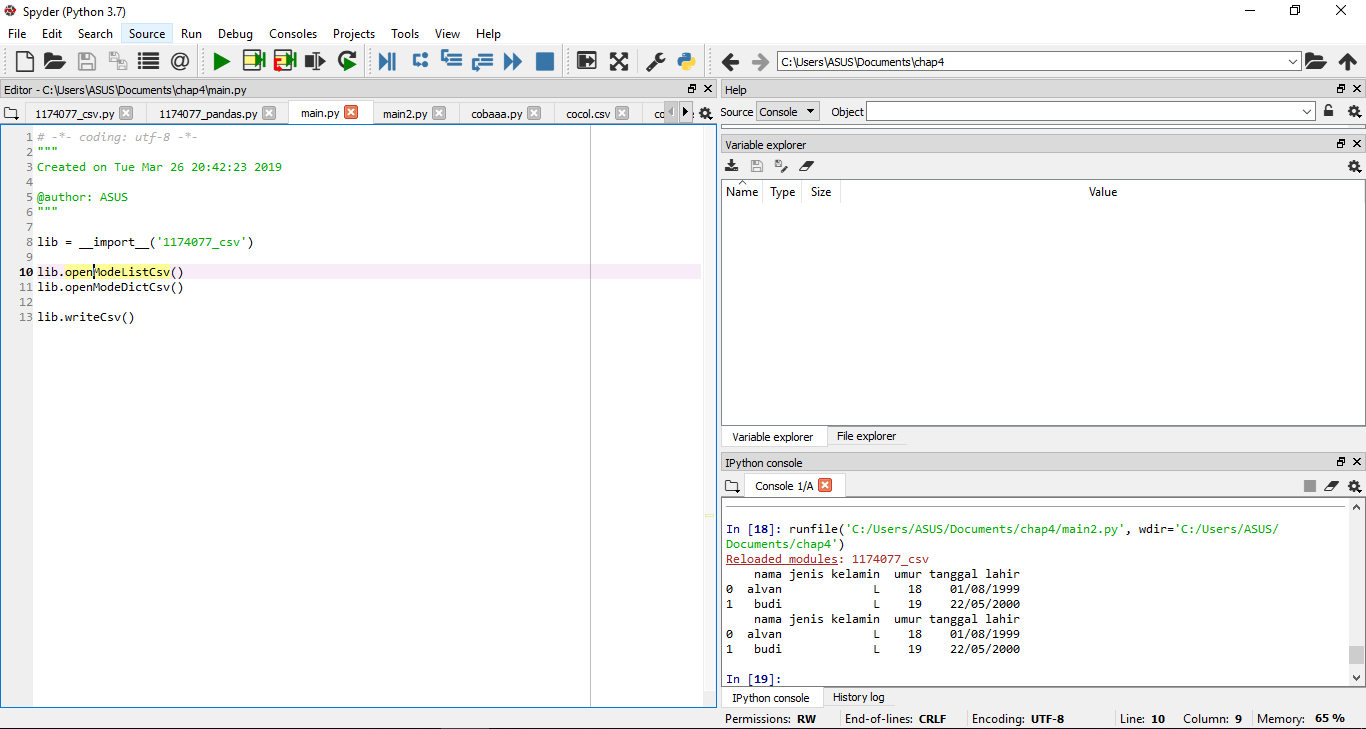
\includegraphics[width=10cm]{figures/4/1174077/Praktek/mainpy.png}
	\centering
\end{figure}
\begin{figure}[!htbp]
	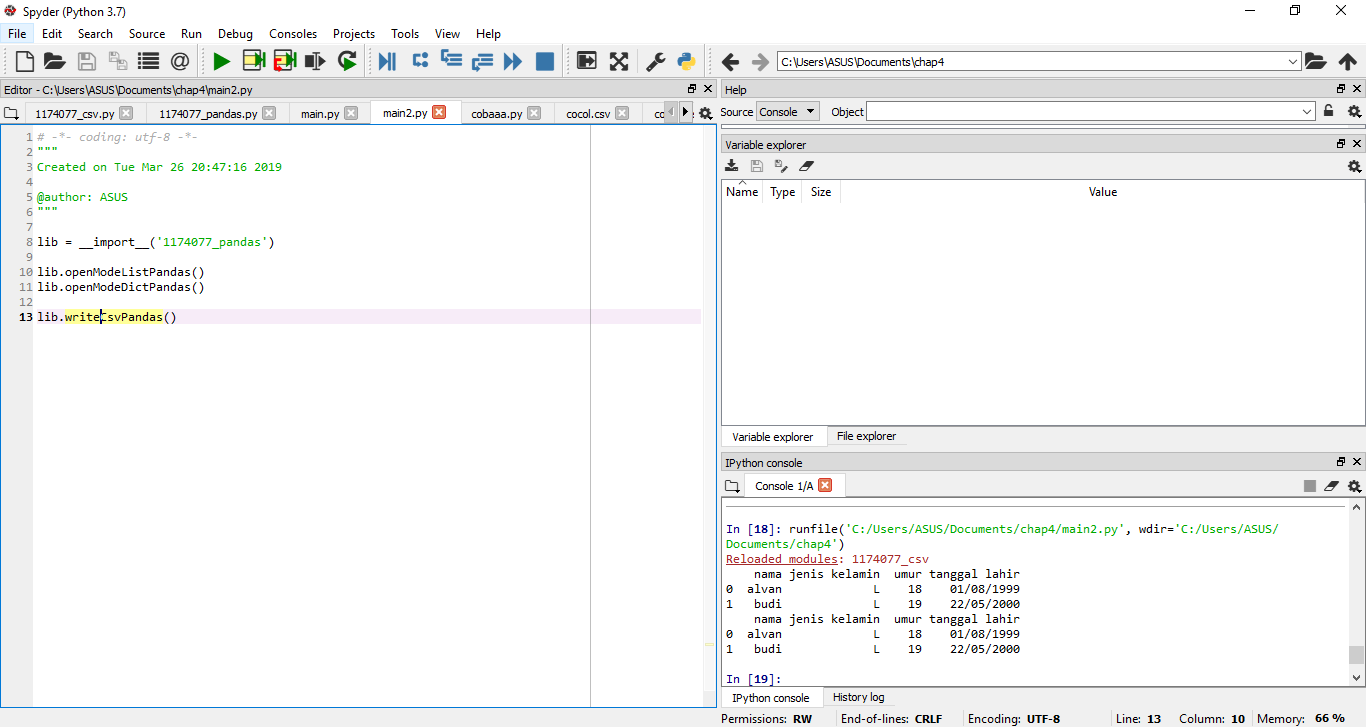
\includegraphics[width=10cm]{figures/4/1174077/Praktek/main2py.png}
	\centering
\end{figure}
\begin{figure}[!htbp]
	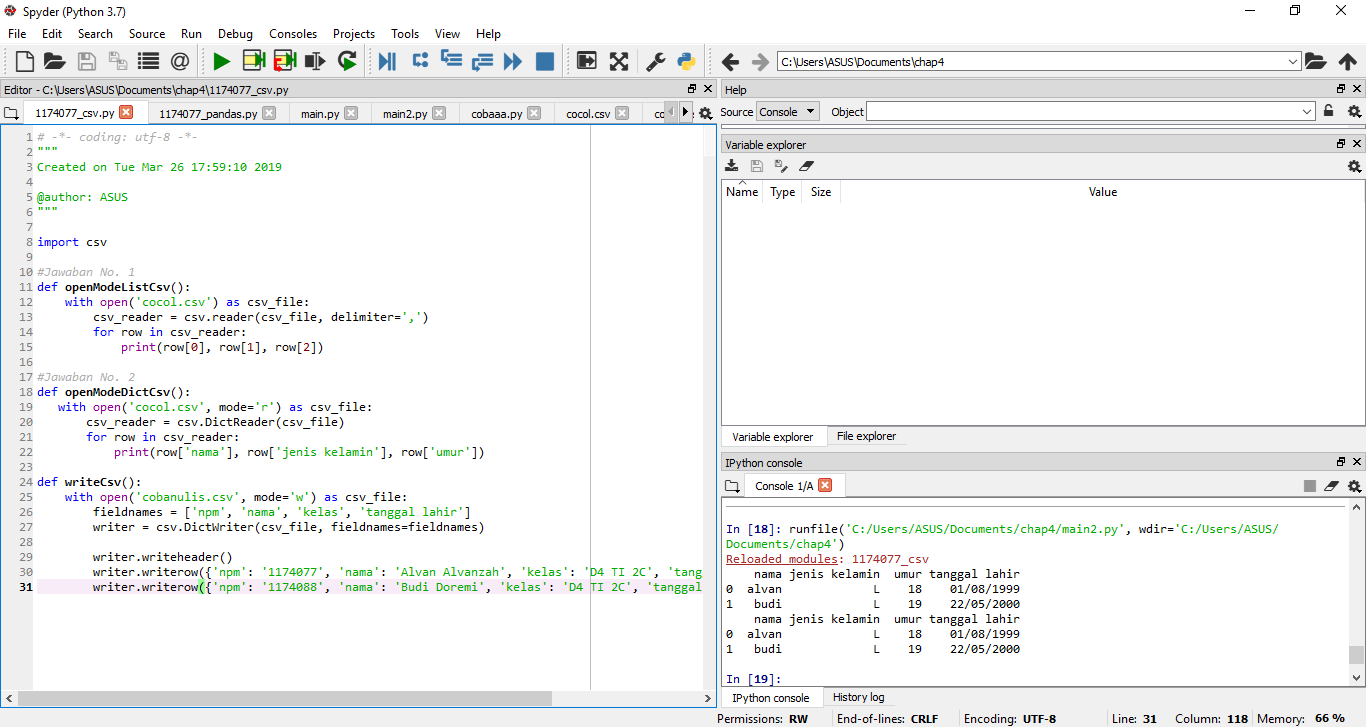
\includegraphics[width=10cm]{figures/4/1174077/Praktek/csv.png}
	\centering
\end{figure}
\begin{figure}[!htbp]
	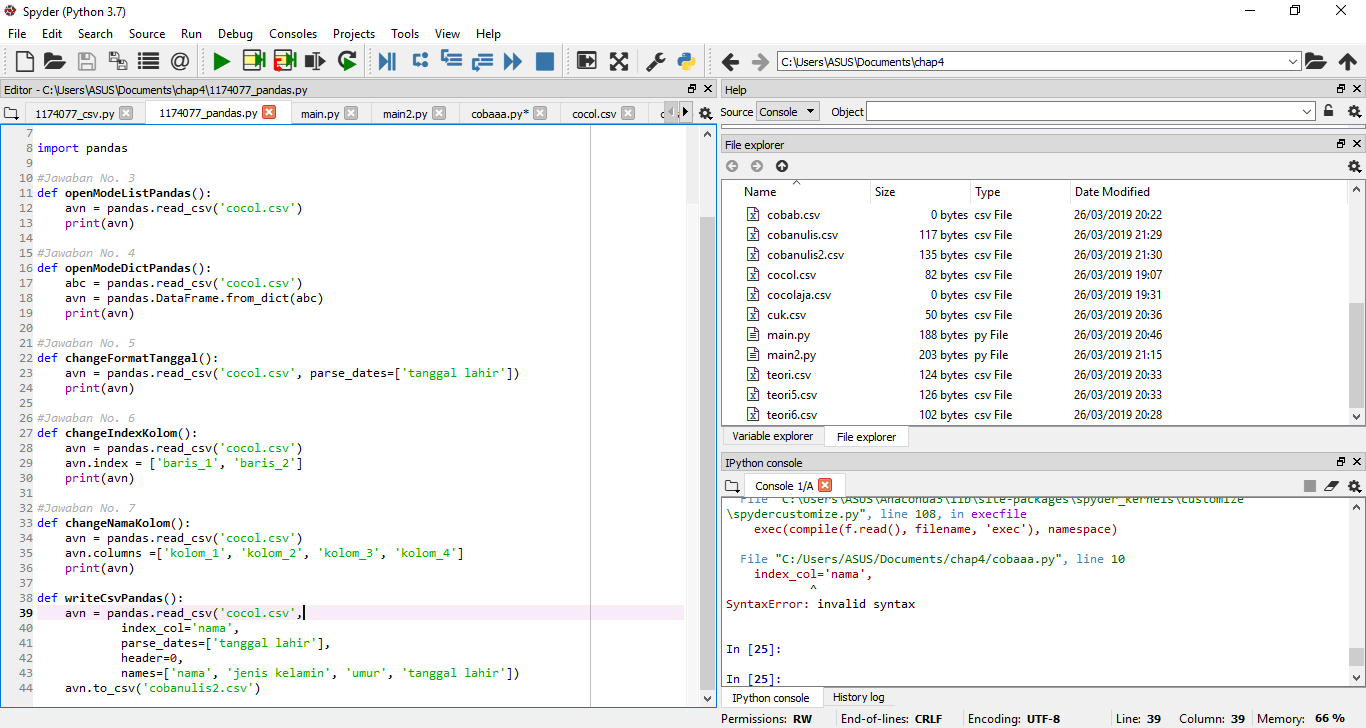
\includegraphics[width=10cm]{figures/4/1174077/Praktek/pandas.png}
	\centering
\end{figure}
%%%%%%%%%%%%%%%%%%%%%%%%%%%%%%%%%%%%%%%%%%%%%%%%%%%%%%%%%%%%%%%%%%%%%%%%%%%%%%%%%%%%%%%%%%%%%%%%%%%%


\title{CHAPTER 4 PRAKTEK}
\author{Handi Hermawan }
\subsection{Keterampilan Pemrograman}
\begin{enumerate}
    \item Buatlah  fungsi  (file  terpisah/library  dengan  nama  \verb|NPM_csv.py|)  untuk  membuka file csv dengan lib csv mode list.
    
   	

    \item Buatlah  fungsi  (file  terpisah/library  dengan  nama  \verb|NPM_csv.py|)  untuk  membuka file csv dengan lib csv mode dictionary.
   	
   	\lstinputlisting[firstline=16, lastline=20]{src/4/1174080/Praktek/1174080_csv.py}

	\item Buatlah fungsi (file terpisah/library dengan nama \verb|NPM_pandas.py|) untuk membuka file csv dengan lib pandas mode list.
	
	\lstinputlisting[firstline=7, lastline=11]{src/4/1174080/Praktek/1174080_pandas.py}
		
	\item Buatlah fungsi (file terpisah/library dengan nama \verb|NPM_pandas.py| untuk membuka file csv dengan lib pandas mode dictionary.

	\lstinputlisting[firstline=13, lastline=16]{src/4/1174080/Praktek/1174080_pandas.py}

	\item Buat fungsi baru di \verb|NPM_pandas.py| untuk mengubah format tanggal menjadi standar dataframe.

	\lstinputlisting[firstline=25, lastline=27]{src/4/1174080/Praktek/1174080_pandas.py}

	\item Buat fungsi baru di \verb|NPM_pandas.py| untuk mengubah index kolom.
	
	\lstinputlisting[firstline=29, lastline=32]{src/4/1174080/Praktek/1174080_pandas.py}
	
	\item Buat fungsi baru di \verb|NPM_pandas.py| untuk mengubah atribut atau nama kolom.
	
	\lstinputlisting[firstline=34, lastline=37]{src/4/1174080/Praktek/1174080_pandas.py}
	
	\item Buat program main.py yang menggunakan library \verb|NPM_csv.py| yang membuat dan membaca file csv.
	
	
	
	\item Buat program main2.py yang menggunakan library \verb|NPM_pandas.py| yang membuat dan membaca file csv.


\end{enumerate} 

\subsection{Keterampilan Penanganan Error}

\begin{enumerate}
	\item Tuliskan peringatan error yang didapat dari mengerjakan praktek ketiga ini,
dan jelaskan cara penanganan error tersebut. dan Buatlah satu fungsi yang
menggunakan gunakan try except untuk menanggulangi error tersebut.
	
	\par NameError adalah exception yang terjadi saat kode melakukan eksekusi terhadap local name atau global name yang tidak terdefinisi. Misalnya saat menjumlahkan variable yang tidak didefinisikan.
	
\end{enumerate}

%%%%%%%%%%%%%%%%%%%%%%%%%%%%%%%%%%%%%%%%%%%%%%%%%%%%%%%%%%%%%%%%%%%%%%%%%%%%%%%%%%%%%%%%%%%%%%%%%%%%%%%%%%%%%


\section{Muhammad Abdul Gani Wijaya}
\subsection{No 1}
Buatlah  fungsi  (file  terpisah/library  dengan  nama  NPMcsv.py)  untuk  membuka file csv dengan lib csv mode list.

\lstinputlisting[caption = Fungsi membuka file CSV dengan lib CSV mode list., firstline=8, lastline=19]{src/4/1174071/Praktek/1174071_csv.py}

\subsection{No 2}
Buatlah  fungsi  (file  terpisah/library  dengan  nama  NPMcsv.py)  untuk  membuka file csv dengan lib csv mode dictionary.

\lstinputlisting[caption =  Fungsi membuka file CSV dengan lib CSV mode dictionary., firstline=21, lastline=30]{src/4/1174071/Praktek/1174071_csv.py}

\subsection{No 3}
Buatlah fungsi (file terpisah/library dengan nama NPMpandas.py) untuk membuka file csv dengan lib pandas mode list.

\lstinputlisting[caption =  Fungsi membuka file CSV dengan lib Pandas mode list., firstline=9, lastline=14]{src/4/1174071/Praktek/1174071_pandas.py}

\subsection{No 4}
Buatlah fungsi (file terpisah/library dengan nama NPMpandas.py) untuk membuka file csv dengan lib pandas mode dictionary.

\lstinputlisting[caption =  Fungsi membuka file CSV dengan lib Pandas mode dictionary., firstline=16, lastline=22]{src/4/1174071/Praktek/1174071_pandas.py}

\subsection{No 5}
Buat fungsi baru di NPMpandas.py untuk mengubah format tanggal menjadi standar dataframe.

\lstinputlisting[caption =  Fungsi mengubah format tanggal menjadi standar dataframe., firstline=24, lastline=29]{src/4/1174071/Praktek/1174071_pandas.py}

\subsection{Soal 6}
Buat fungsi baru di NPMpandas.py untuk mengubah index kolom.

\lstinputlisting[caption =  Fungsi mengubah index kolom., firstline=31, lastline=37]{src/4/1174071/Praktek/1174071_pandas.py}

\subsection{Soal 7}
Buat fungsi baru di NPMpandas.py untuk mengubah atribut atau nama kolom.

\lstinputlisting[caption =  Fungsi untuk mengubah atribut atau nama kolom., firstline=26, lastline=30]{src/4/1174071/Praktek/1174071_pandas.py}

\subsection{Soal 8}
Buat program main.py yang menggunakan library NPMcsv.py yang membuat dan membaca file csv.

\lstinputlisting[caption =  Membuat dan membaca file CSV menggunakan library 1174071pandas., firstline=8, lastline=13]{src/4/1174071/Praktek/main.py}

\subsection{Soal 9}
Buat program main2.py yang menggunakan library NPMpandas.py yang membuat dan membaca file csv.

\lstinputlisting[caption = Membuat dan mmebaca file CSV menggunakan library 1174071pandas., firstline=8, lastline=13]{src/4/1174071/Praktek/main2.py}

\subsection{Kode Program Praktek}
\begin{figure}[ht]
	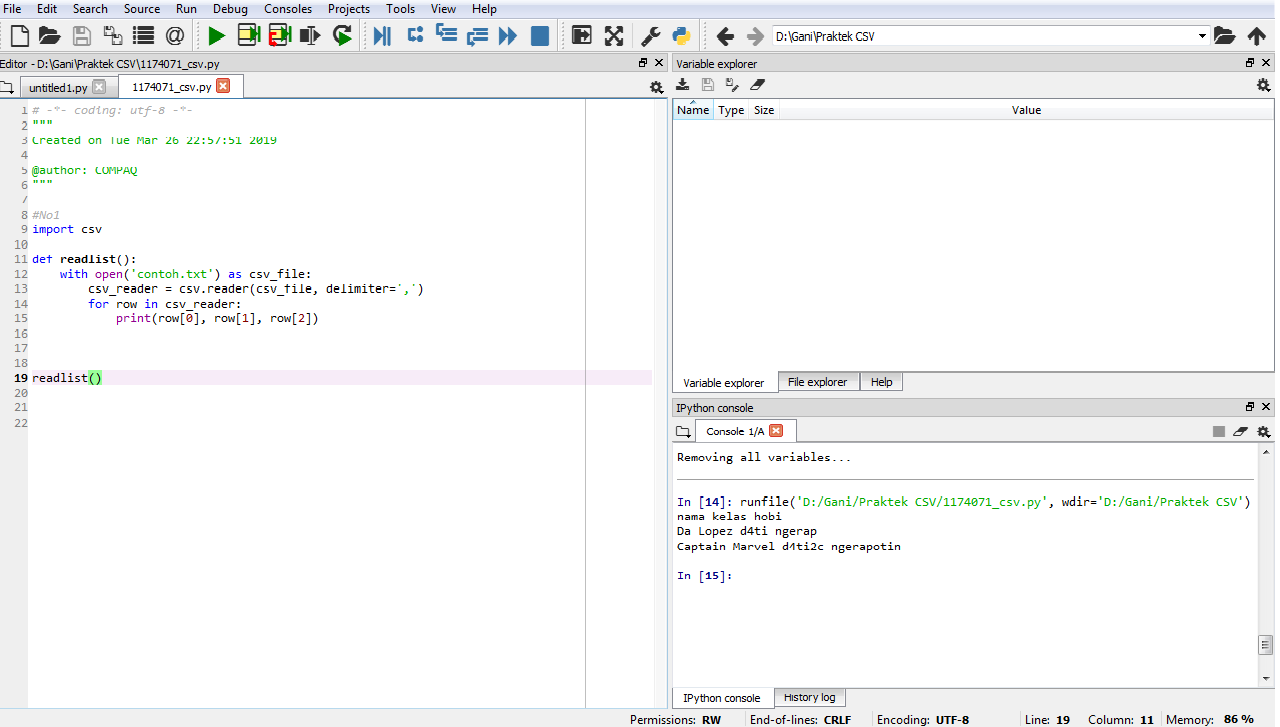
\includegraphics[width=9cm]{figures/4/1174071/Praktek/1174071_csv1.png}
	\centering
\end{figure}
\begin{figure}[ht]
	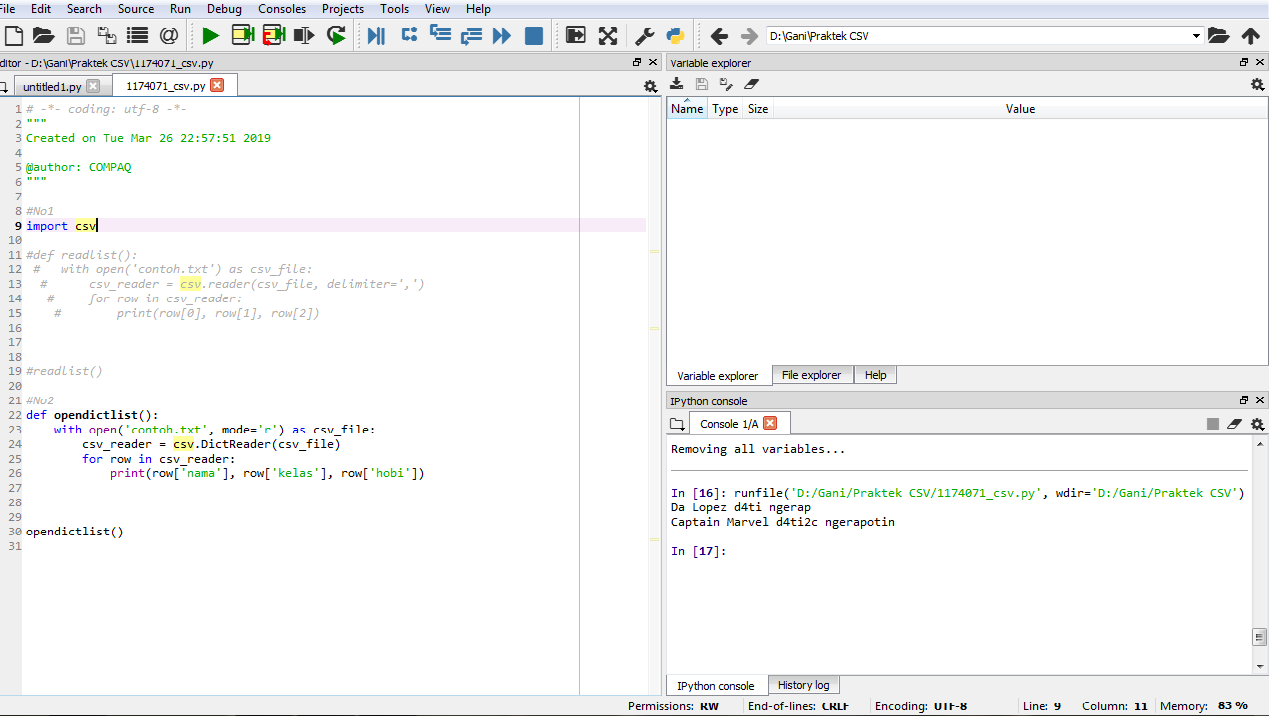
\includegraphics[width=10cm]{figures/4/1174071/Praktek/1174071_csv2.png}
	\centering
\end{figure}
\begin{figure}[ht]
	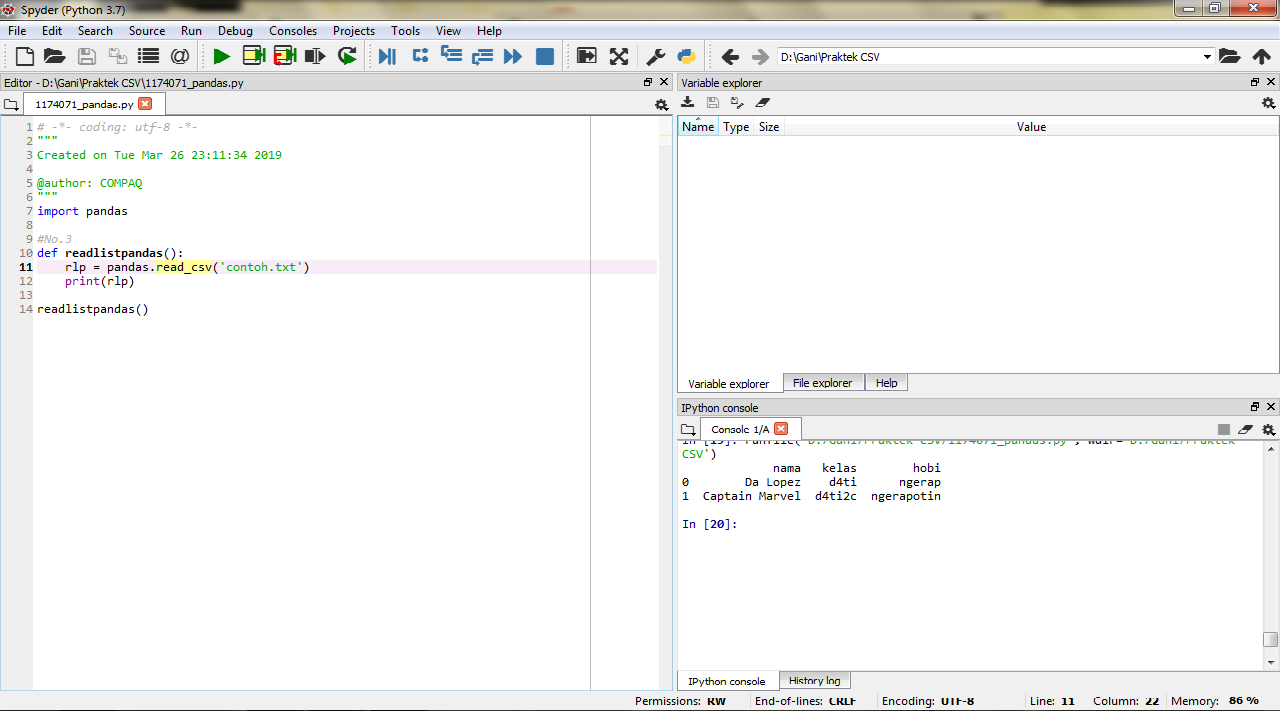
\includegraphics[width=10cm]{figures/4/1174071/Praktek/1174071_pandas3.png}
	\centering
\end{figure}
\begin{figure}[ht]
	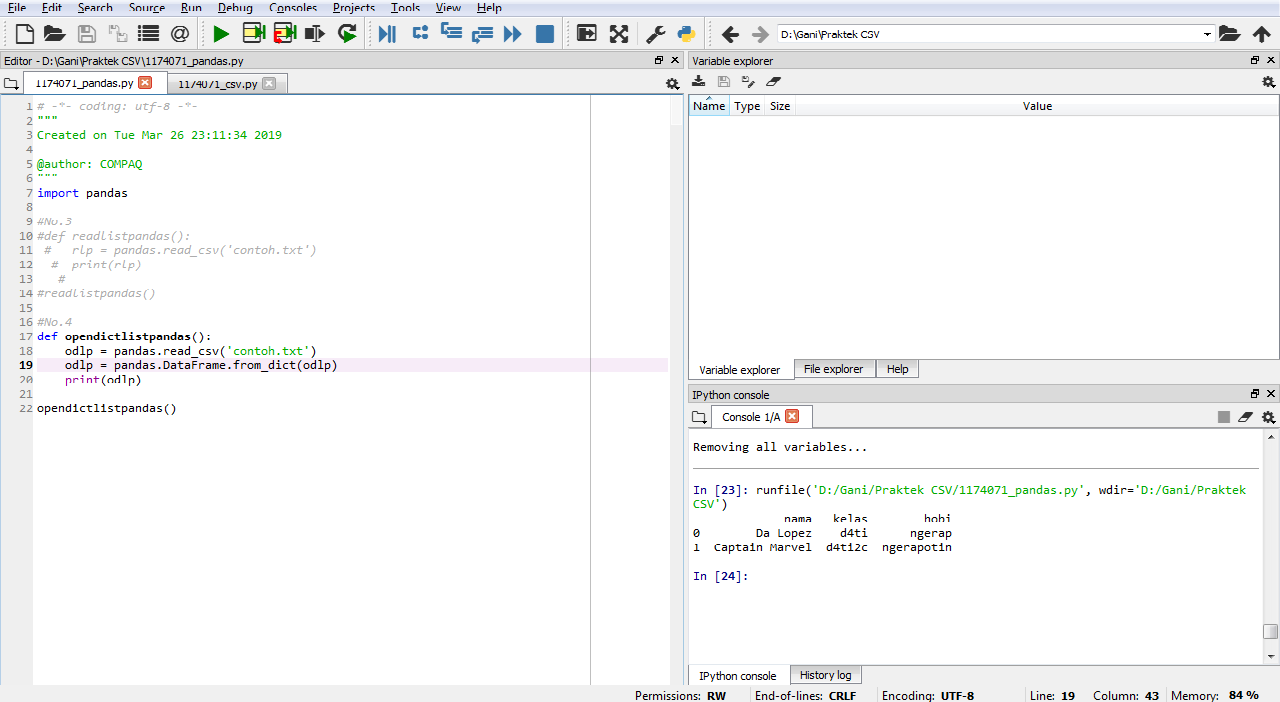
\includegraphics[width=9cm]{figures/4/1174071/Praktek/1174071_pandas4.png}
	\centering
\end{figure}
\begin{figure}[ht]
	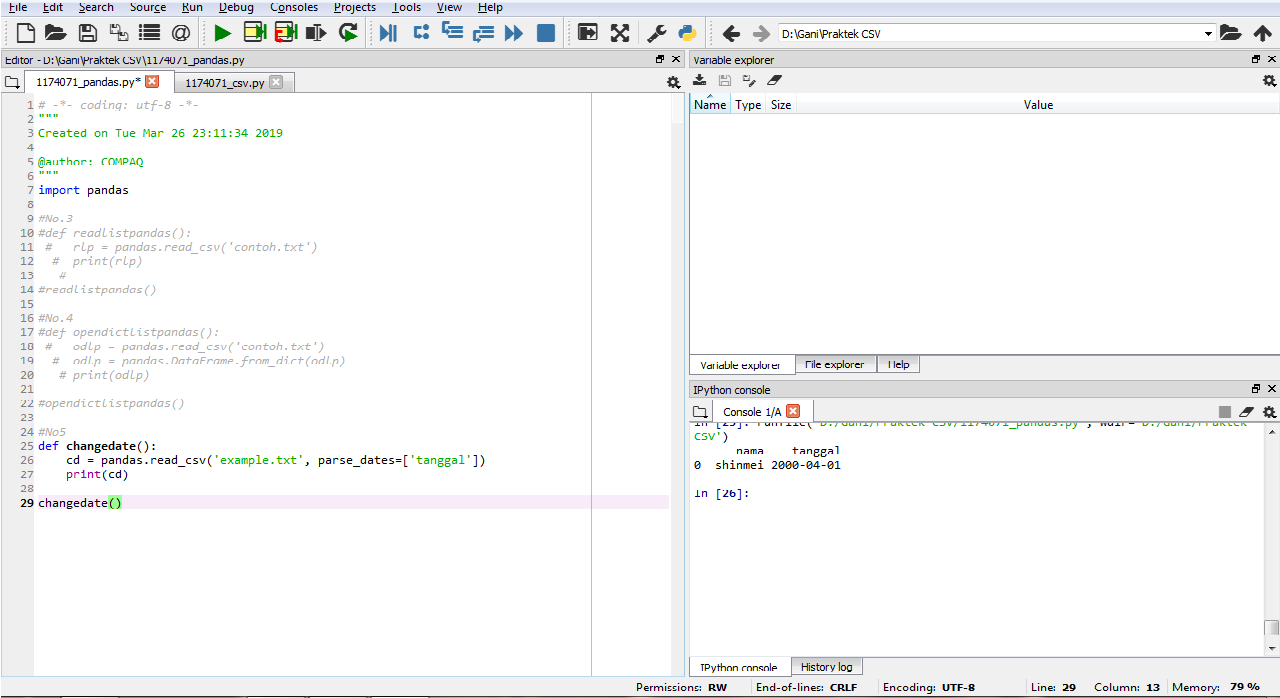
\includegraphics[width=10cm]{figures/4/1174071/Praktek/1174071_pandas5.png}
	\centering
\end{figure}
\begin{figure}[ht]
	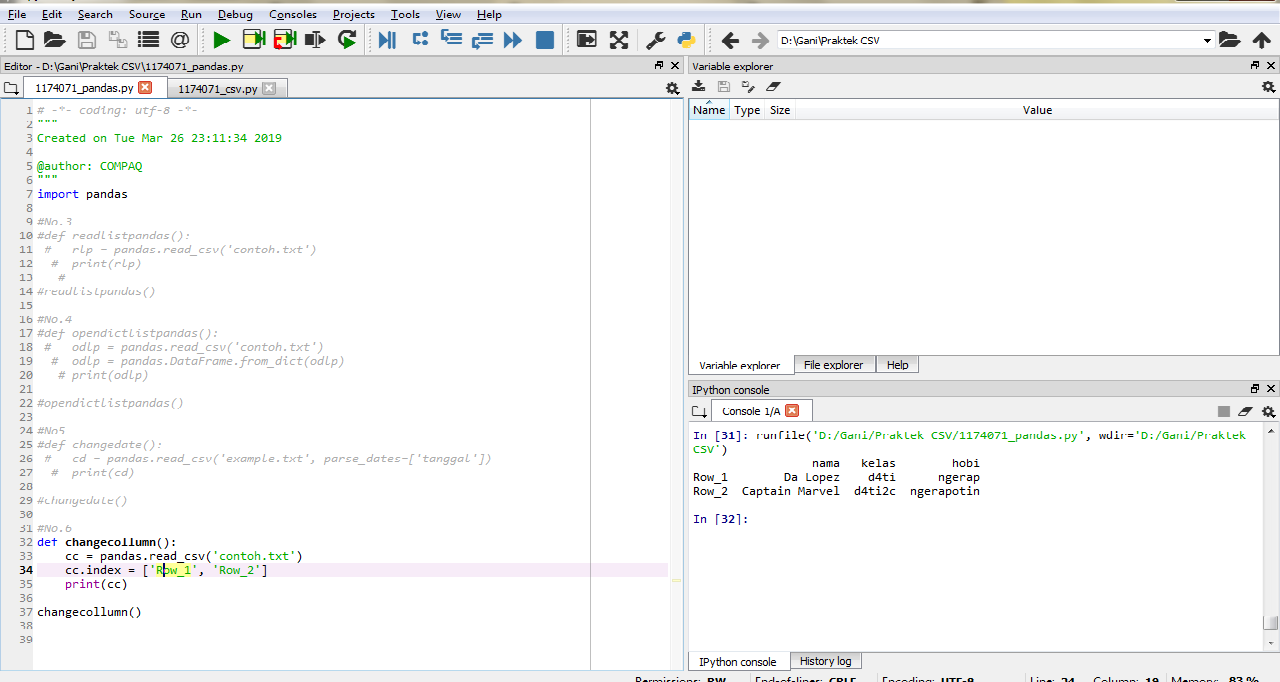
\includegraphics[width=10cm]{figures/4/1174071/Praktek/1174071_pandas6.png}
	\centering
\end{figure}
\begin{figure}[ht]
	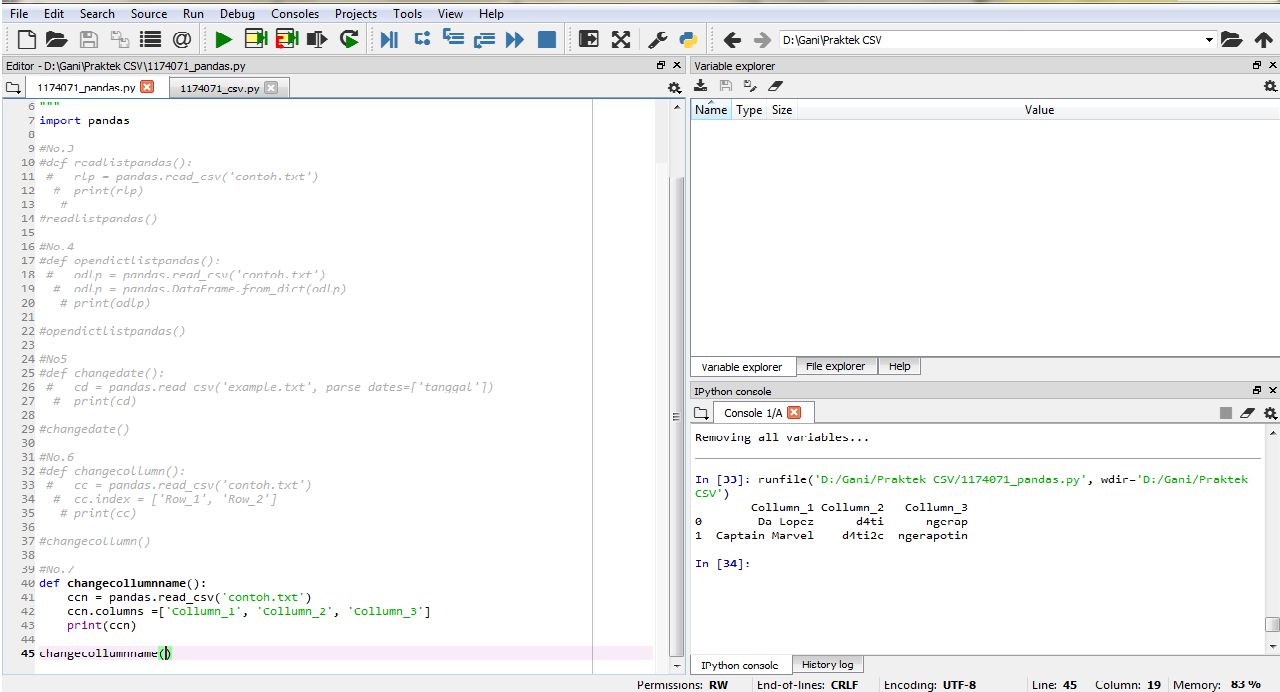
\includegraphics[width=10cm]{figures/4/1174071/Praktek/1174071_pandas7.png}
	\centering
\end{figure}
\begin{figure}[ht]
	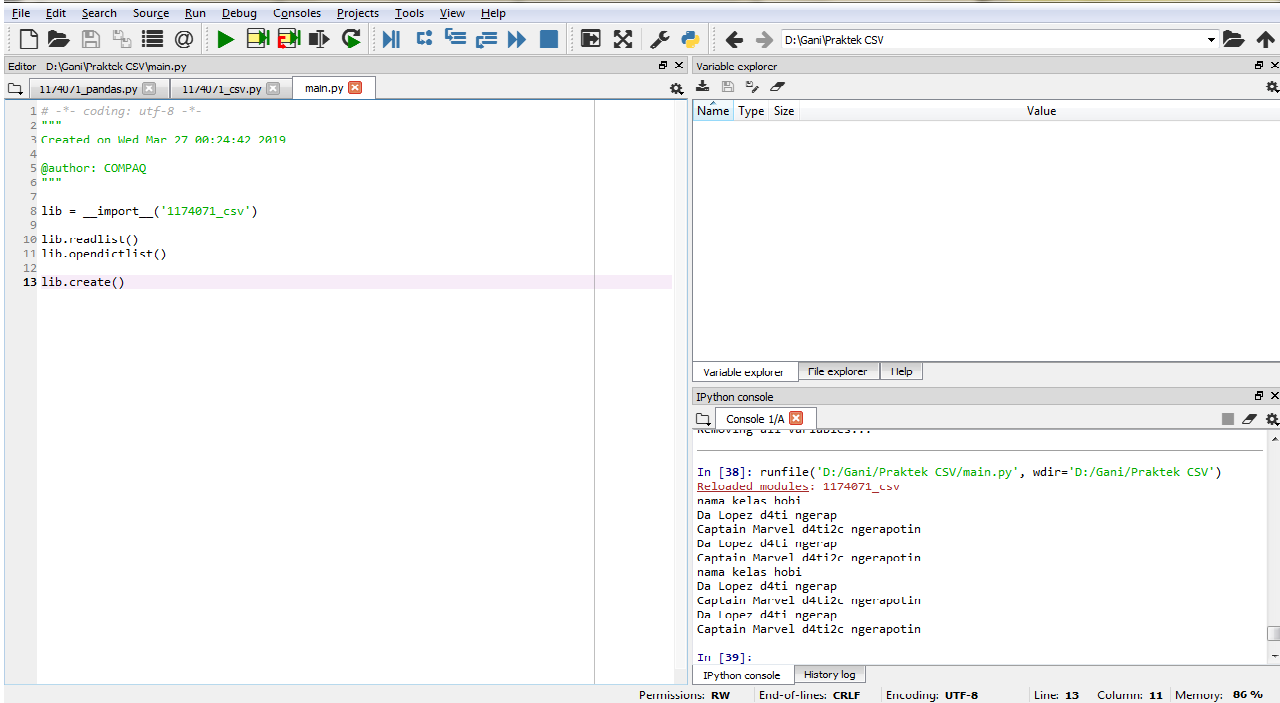
\includegraphics[width=10cm]{figures/4/1174071/Praktek/1174071_main8.png}
	\centering
\end{figure}
\begin{figure}[ht]
	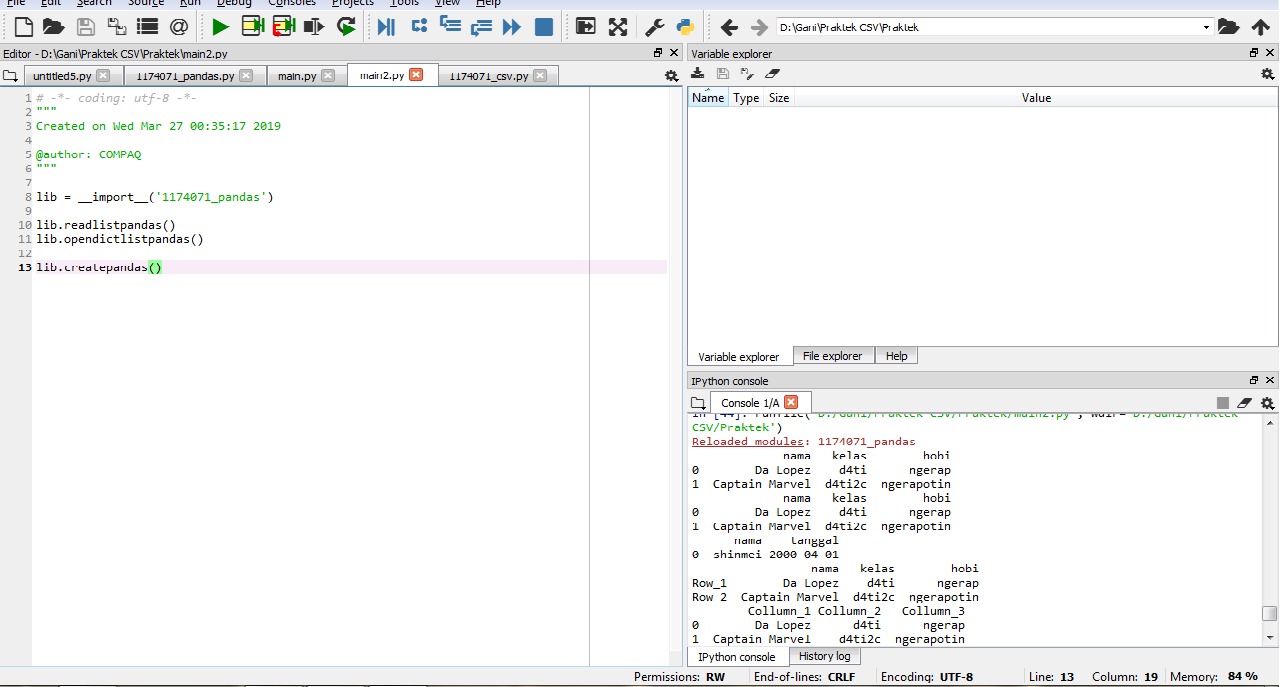
\includegraphics[width=10cm]{figures/4/1174071/Praktek/1174071_main9.png}
	\centering
\end{figure}


%%%%%%%%%%%%%%%%%%%%%%%%%%%%%%%%%%%%%%%%%%%%%%%%%%%%%%%%%%%%%%%%%%%%%%%%%%%%%%%%%%%%%%%%%%%%%%%%%%%%%



%TEORI
%\chapter{Komumikasi Perangkat keras}
%%\section{Tomy Prawoto}
%\subsection{Soal 1}
%Isi jawaban soal ke-1

%Kalau mau dibikin paragrap \textbf{cukup enter aja}, tidak usah pakai \verb|par| dsb

%\subsection{Soal 2}
%Isi jawaban soal ke-2

%\subsection{Soal 3}
%Isi jawaban soal ke-3

%%%%%%%%%%%%%%%%%%%%%%%%%%%%%%%%%%%%%%%%%%%%%%%%%%%%%%%%%%%%%%%%%%%%%%%%%%%%%%%%%%%%%%%%%%%%%%%%%%%

\section{Kaka Kamaludin}
\subsection{Soal 1}
folder /dev pada linux beriisi file konfigurasi hardware.
Device Manager berfungsi untuk mengatur driver hardware.

\subsection{Soal 2}
\begin{itemize}
	\item download Arduino Software(IDE)  
		https://www.arduino.cc/en/Main/Software
		download untuk linux
	\item extract file yang di download dan masuk ke folder hasil extract
	\item jalankan "./install.sh"
\end{itemize}

\subsection{Soal 3}
. . .

\subsection{Soal 4}
modul pyserial berfungsi untuk merangkum akses untuk port serial. moduk ini dapat di gunakan untuk python yang berjalan pada windows, osx, BSD (yang mendukung system POSIX) dan IronPython.Ini dirilis di bawah lisensi perangkat lunak gratis.

\subsection{Soal 5}
\begin{itemize}
	\item serial.Serial('/dev/tty*')
	membuka port serial
	
	\item ser.close()
	menutup port serial
	
	\item ser.read()
	membaca satu bit
	
	\item ser.readline()
	membaca line semua line
		
\end{itemize}

\subsection{Soal 6}
fungsi perulangan dibutuhkan untuk penggunaan code membutuhkan penggunaan contoh nya seperti multiple choce yang menggunakan perulangan tak terhingga 'while'.

\subsection{Soal 7}
\lstinputlisting[firstline=1, lastline=9]{src/5/1174067/Teori/1174067.py}

%%%%%%%%%%%%%%%%%%%%%%%%%%%%%%%%%%%%%%%%%%%%%%%%%%%%%%%%%%%%%%%%%%%%%%%%%%%%%%%%%%%%%%

\section{Ainul Filiani}
\begin{enumerate}
\item Apa itu fungsi device manager di windows dan folder /dev linux ?

Device Manager pada komputer Windows atau linux, diambil dari Microsoft Management Console. Pengelola Perangkat Menampilkan semua perangkat keras yang dapat diinisialisasi (dikenali) oleh Windows atau linux. Penampilan telah diatur (dikelompokkan) sehingga akan memudahkan pengelolaan setiap perangkat keras yang ada.
Pengelola Perangkat Windows atau linux
Device Manager akan sangat membantu dalam mengelola (mengelola) semua perangkat keras yang diinstal (dan diinstal) dalam sistem Windows atau linux. Perangkat keras seperti hard drive, kartu VGA, suara, keyboard, perangkat USB dll. Akan sangat mudah untuk mengaksesnya dari dalam Device Manager.

Beberapa fungsi kegunaan Manajer Perangkat meliputi:
\begin{enumerate}
\item Membahas status perangkat perangkat keras
\item Diskusikan informasi terperinci tentang perangkat keras
\item Kelola driver perangkat keras
\item Nonaktifkan dan Aktifkan perangkat keras
\item Mengatasi konflik perangkat keras, dll.
\end{enumerate}

\item Jelaskan Langkah-Langkah Instalasi Driver Dari Arduino ?

\begin{enumerate}
\item Menginstal Arduino IDE pada perangkat Windows: 

Karena file IDE Arduino yang dipilih dalam unduhan sebelumnya adalah format file .zip, file ini tidak memerlukan instalasi untuk digunakan, dengan kata lain, ini adalah file IDE Arduino yang portabel.
\item Pertama, silakan sambungkan Arduino ke PC Windows 10 atau laptop Anda menggunakan kabel USB
\item Setelah itu, buka Device Manager. Caranya adalah dengan hanya menekan tombol Windows + Pause Break secara bersamaan, lalu pilih Device Manager di menu sebelah kiri
\item Ketika Anda telah memasuki tampilan Device Manager, silakan pilih Ports (COM dan LPT). Setelah dipilih akan muncul drop down yang bertuliskan USB Serial Device (COM4)
\item Klik kanan pada bagian USB Serial Device (COM4), lalu pilih Update Driver
\item Setelah dua pilihan muncul, silakan pilih Browse my computer for software driver
\item Langkah selanjutnya silakan cari di mana folder Anda menyimpan driver Arduino. Karena itu, pastikan Anda memiliki driver. Jika Anda tidak memilikinya, silakan unduh terlebih dahulu
\item Setelah Anda memilih folder lokasi driver Arduino, silakan klik OK dan tunggu sampai proses instalasi driver selesai
\item Jika proses instalasi selesai dan berhasil, maka penulisan USB Serial Device (COM4) di Device Manager akan berubah menjadi Arduino Uno (COM4) atau seri lain sesuai dengan Arduino yang Anda gunakan
\item terakir Anda bisa langsung memasukkan program ke Arduino dari komputer

\end{enumerate}
\item Jelaskan bagaimana cara membaca baudrate dan port dari komputer yang sudah terinstall driver ? 

Untuk membaca baudrate bisa dicek melalui arduino IDE, setelah itu  untuk mengecheck port dapat dilakukan dengan device manager


\item Jelaskan sejarah library pyserial ? 

Modul ini merangkum akses untuk port serial. Ini menyediakan backends untuk Python yang berjalan di Windows, Linux, BSD (mungkin sistem yang mendukung POSIX), Jython dan IronPython (.NET dan Mono). Modul bernama "serial" secara otomatis memilih backend yang sesuai. Antarmuka berbasis kelas yang sama pada semua platform yang didukung.
Akses ke pengaturan port melalui properti Python.
Dukungan untuk berbagai ukuran byte, bit stop, paritas dan kontrol aliran dengan RTS / CTS dan / atau Xon / Xoff.
Bekerja dengan atau tanpa menerima batas waktu.
File seperti API dengan "read" dan "write" ("readline" dll. Juga didukung).
File-file dalam paket ini adalah 100 persen Python murni.
Port diatur untuk transmisi biner. Tidak ada stripping byte NULL, terjemahan CR-LF dll. (Yang berkali-kali diaktifkan untuk POSIX.) Ini membuat modul ini bermanfaat secara universal.
Kompatibel dengan pustaka io (Python 2.6+)

\item Jelaskan fungsi apa saja yang dipakai library pyserial ?
\begin{enumerate}
\item ‘A’	RELAY ON
\item ‘Z’	RELAY OFF
\item ‘1’	RELAY ON selama 100ms
\item ‘2’	RELAY ON selama 250ms
\item ‘3’	RELAY ON selama 500ms


\end{enumerate}
\item Jelaskan kenapa perlu pengulangan dalam tidak butuh perulangan dalam membaca serial ? 

Perualangan dalam bahasa pemrograman berfungsi menyuruh komputer melakukan sesuatu secara berulang-ulang. Terdapat dua jenis perualangan dalam bahasa pemrograman python, yaitu perulangan dengan for dan while.
Perulangan for disebut counted loop (perulangan yang terhitung), sementara perulangan while disebut uncounted loop (perulangan yang tak terhitung). Perbedaannya adalah perulangan for biasanya digunakan untuk mengulangi kode yang sudah diketahui banyak perulangannya. Sementara while untuk perulangan yang memiliki syarat dan tidak tentu berapa banyak perulangannya.
Perulangan diperlukan agar dapat membaca data secara berulang kali sehingga data yang muncul lebih dari satu.  Sedangkan apabila tidak memakai perulangan maka data akan terbaca satu kali saja.
\item Jelaskan cara membuat fungsi yang menggunakan pyserial ? 

Sebelum dapat menggunakan fungsi-fungsi PySerial dalam program, kita harus meng-import-nya terlebih dahulu dengan perintah:
import serial
Setelah itu  kita bisa mem-binding object SER2REL dengan port serial COM1 pada baudrate 2400.
SER2REL = serial.Serial(“COM1”, 2400)
Apabila  binding berhasil maka port serial COM1 akan di-open dan siap digunakan. Untuk mengetes apakah COM1 sudah open dan siap digunakan, kita gunakan fungsi isOpen sebagai berikut:
SER2REL.isOpen()
Fungsi ini menghasilkan nilai True jika COM1 sudah open dan nilai False jika sebaliknya. Pada eksperimen kita, SER2REL.isOpen() menghasilkan nilai True yang berarti kita sudah dapat mengirim dan menerima data ke dan dari port serial COM1.
Untuk mengaktifkan RELAY-1, kita harus mengirimkan karakter ‘A’ ke modul SER-2REL. Perintah yang digunakan adalah:
SER2REL.write(“AAA”)
Pada perintah tersebut kita tidak mengirimkan 1 buah karakter ‘A’ melainkan 3 buah karakter ‘A’. Mengapa? Untuk safety saja. Siapa tahu ada kesalahan transmisi.  
Modul SER-2REL menggunakan kristal 11.0592MHz untuk meyakinkan bahwa clock baudrate untuk port serial memiliki kesalahan nol persen.
Perintah-perintah selanjutnya adalah perintah-perintah untuk:
\begin{enumerate}
\item mematikan RELAY-1
\item mengaktifkan RELAY-2
\item mematikan RELAY-2
\item mengaktifkan kedua relay secara bersamaan
\item dan mematikan kedua relay secara bersamaan.
\end{enumerate}

Berikut adalah skrip Python  yang disimpan dalam bentuk file program SER-2REL.py.

\#\_\_\_\_\_\_\_\_\_\_\_\_\_\_\_\_\_\_\_\_\_

\# Name:         SER-2REL.PY 

\# Purpose:      Program Kontrol Pengujian Modul SER-2REL 

\# Author:       Chandra MDE 

\# Created:      17/04/2013 

\# Copyright:    (c) Chandra MDE 2013 

\#\_\_\_\_\_\_\_\_\_\_\_\_\_\_\_\_\_\_\_\_\_



-import serial, time 
def main(): 

    ser2rel = serial.Serial("COM1", 2400) 
    
    if not ser2rel.isOpen(): 
    
        ser2rel.open() 
        
    print "RELAY-1 ON" 
    
    ser2rel.write(‘AAA’)    \#RELAY-1 ON 
    
    time.sleep(1) 
    
    print "RELAY-1 OFF" 
    
    ser2rel.write(‘XXX’)    \#RELAY-1 OFF 
    
    time.sleep(1) 
    
    print "RELAY-2 ON" 
    
    ser2rel.write(‘BBB’)    \#RELAY-2 ON 
    
    time.sleep(1) 
    
    print "RELAY-2 OFF" 
    
    ser2rel.write(‘YYY’)    \#RELAY-2 OFF 
    
    time.sleep(1) 
    
    print "RELAY-1 dan RELAY-2 ON" 
    
    ser2rel.write(‘CCC’)    \#ALL ON 
    
    time.sleep(1) 
    
    print "RELAY-1 dan RELAY-2 OFF" 
    
    ser2rel.write(‘ZZZ’)    \#ALL OFF 
    
    time.sleep(1) 
    
    if ser2rel.isOpen(): 
    
        ser2rel.close() 
        
        if\_\_name\_\_== '\_\_main\_\_':
        
        main()





\end{enumerate}
%%%%%%%%%%%%%%%%%%%%%%%%%%%%%%%%%%%%%%%%%%%%%%%%%%%%%%%%%%%%%%%%%%%%%%%%%%%%%%%%%%%%%%%%%%
\section {Sekar Jasmine}
\begin{enumerate}

\item 1. Apa itu fungsi device manager di windows dan folder.
Device Manager adalah applet Panel Kontrol dalam sistem operasi Microsoft windows , ini  memungkinkan pengguna untuk melihat dan mengontrol perangkat keras yang terpasang pada komputer. ketika sepotong perangkat keras tidak berfyngsi. , perangkat keras yang menyinggung disorot bagi pengguna untuk berurusan dengan daftar perangkat keras dapat diurutkan berdasarkan berbagai kriteria.\\

untuk setiap perangkat , pengguna dapat menyediakan driver perangkat sesuai dengan model driver windows , aktifkan atau nonaktifkan perangkat.\\

\item 2. Jelaskan langkah-langkah instalasi driver dari arduino.
1. pasang board Arduino anda ke port USB pada komputer atau laptop , kemudian tunggu hingga windows mencoba untuk menginstall driver sendiri.\\
2. jika berhasil , berati instalasi selesai tapi jika gagal lanjutkan ke step berikutnya.
3. Anda harus menginstall dari device manager untuk masuk ke device manager anda bisa melakukan dengan 2 cara .\\
Cara 1 . A tekan tombol windows tambah R secara bersamaan. setelah itu tombol windows adalah tombol pada keyboard dengan logo windows. setelah anda menekan tombol windows plus R maka akan muncul Run ketikkan devmgmt.msc kemudian tekan tombol ENTER.
cara 2 . B Klik start - pilih control panel . di dalam control panel pilih system dan security lalu pilih system , selanjutnya pilih Device Manager.\\

\item 3. Jelaskan bagaimana cara membaca baudrate dan port dari komputer yang sudah terinstall driver.
Pada komunikasi dengan kabel yang panjang , masalah kabel loss tidak akan menjadi masalah besar daripada menggunakan kabel level tegangan -3 vlot sampai -25 vlot dan 0.

dalam komunikasi data serial dengan cara asinkron , kecepatan pengiriman data (baudrate) dan fase clock pada sisi transmiter dan pada sisi receiver harus sinkron. Untuk itu diperlukan sinkronisasi antara transmitter dan receiver.\\

kecepatan baudrate dapat dipilih bebas dalam rentang nilai yang umum digunakan adalah 110 , 135 , 150 , 300 , 600 , 1200 , 2400 dan 9600 (bit/detik). dalam komunikasi data serial baudrate dari kedua alat yang berhubungan harus diatur pada kecepatan yang sama.\\

\item 4. Jelaskan sejarah library pyserial.
jadi library pyserial dibuat ke port tersebut ia meneruskan semua data ke port serial dan sebaliknya. Contohnya hanya mengekspor koneksi soket mentah , conthnya berikut dibawah ini memberikan client lebih banyak kontrol atas port serial jarak jauh.\\

for( int hitungan = 0; hitungan <= 10; hitungan++ ){
    // blok kode yang akan diulang
}

class Bintang{
    public static void main(String[] args){

        for(int i=0; i <= 5; i++){
            System.out.println("*****");
        }

    }
}
Pengaturan serial diatur pada baris perintah saat memulai program. tidak ada kemungkinan untuk mengubah pengaturan dari jarak jauh semua data dilewatkan apa adanya.\\

library/modul Python siap-pakai dan gratis yang dibuat untuk memudahkan kita dalam membuat program komunikasi data serial RS232 dalam bahasa Python.\\

\item 5. Jelaskan fungsi-fungsi apa saja yang dipakai dari library pyserial.
A. Import serial untuk membinding object ser2rel dengan port serial com1 pada baudrate 2400.\\

SER2REL untuk binding hasil maka port serial COM1 akan di-open dan siap digunakan untuk mengetes apakah COM1 sudah open dan siap digunakan fungsi isopen sebagai berikut :
A. SER2REL.isOpen fungsi ini menghasilkan nilai true jika COM1 sudah open dan nilai false jika sebaliknya.\\
Untuk mengaktifkan RELAY-1 , kita harus mengirimkan karakter 'A' ke modul SER-2REL.\\

B. SER2REL.Write untuk menggunakan kristal 11.0592MHz untuk menyakinkan bahwa clock baudrate untuk port serial memiliki kesalahan nol persen.\\

\item 6. Jelaskan kenapa butuh perulanggan dalam tidak butuh perulanggan dalam baca serial.
Perulangan atau dalam istilah lain disebut dengan loop. Perulangan digunakan ketika kamu harus menyelesaikan sebuah task dengan jumlah yang besar dengan menggunakan pola yang sama.\\
kalau tidak butuh perulangan maka tidak akan jalan/dibaca program yang anda bikin ,karena perulangan itu sangat butuh untuk mengetahui dimana letak for , while , do while . dll.\\

\item 7. Jelaskan bagaimana cara membuat fungsi yang menggunakan pyserial.
import serial untuk Selanjutnya kita dapat mem-binding object SER2REL dengan port serial COM1 pada baudrate 2400.\\

SER2REL = serial.Serial(“COM1”, 2400)
Jika binding berhasil maka port serial COM1 akan di-open dan siap digunakan. Untuk mengetes apakah COM1 sudah open dan siap digunakan, kita gunakan fungsi isOpen sebagai berikut:
A. SER2REL.isOpen()
Fungsi ini menghasilkan nilai True jika COM1 sudah open dan nilai False jika sebaliknya. Pada eksperimen kita, SER2REL.isOpen() menghasilkan nilai True yang berarti kita sudah dapat mengirim dan menerima data ke dan dari port serial COM1.\\

B. SER2REL.write(“AAA”)
SER-2REL menggunakan kristal 11.0592MHz untuk meyakinkan bahwa clock baudrate untuk port serial memiliki kesalahan nol persen.\\

Perintah-perintah selanjutnya adalah perintah-perintah untuk:

mematikan RELAY-1
mengaktifkan RELAY-2
mematikan RELAY-2
mengaktifkan kedua relay secara bersamaan
dan mematikan kedua relay secara bersamaan.\\

\end{enumerate}
%%%%%%%%%%%%%%%%%%%%%%%%%%%%%%%%%%%%%%%%%%%%%%%%%%%%%%%%%%%%%%%%
\section{Alvan Alvanzah/1174077}
\subsection{Pemahaman Teori}
\begin{enumerate}
    \item Apa itu fungsi device manager di windows dan folder /dev di linux.
    \begin{itemize}
        \item Device  Manager berfungsi untuk membantuk dalam mengelola semua hardware yang terpasang dalam suatu sistem windows. Contohnya seperti harddisk, kartu VGA, sound, keyboard, perangkat USB dll. Akan mudah dikonfiguarsi dari dalam device manager.
        \item Folder /dev berfungsi untuk menyimpan seluruh informasi yang tersimpan dalam linux berada pada sebuah struktur file.
    \end{itemize}
    
    \item Jelaskan langkah-langkah instalasi driver dari arduino.
    \begin{itemize}
        \item Pertama hubungkan sistem minimum Arduino Uno ke komputer atau laptop dengan kabel USB type B.
        \item Lalu pada begian kanan desktop PC anda, akan muncul pop up "Installing device driver software".
        \item Sistem operasi windows tidak menyediakan driver untuk Arduiono Uno, lalu proses instalasinyan harus dilakukan secara manual.
        \item Kemudian buka device manager, dengan caranya pada bagian search program and files lalu ketikkan ”device manager”. Pada control panel akan muncul device manager, klik untuk menjalankan.
        \item Cari unknown device pada bagian other device, lihat tanda seru berwarna kuning, itu disebabkan karena penginstallan tidak berjalan dengan sempurna.
        \item Klik kanan pada "unknown device" kemudian pilih Update Driver Software.
        \item Pilih Browse my computer for driver software.
        \item Arahkan lokasi folder ke file drver arduinonya. Pastikan check-box dicentang include subfolders. Klik next untuk melanjutkan instalasi driver.
        \item Kemudian lanjutkan dengan mengklik install pada tampilan windows security.
        \item Jika instalasi driver berhasil maka akan muncul windows has succesfully updated your driver software.
        \item Perhatikan dan ingat nama COM Arduino Uno, karena nama COM ini yang akan digunakan untuk meng-upload program nantinya.
    \end{itemize}
    
    \item Jelaskan bagaimana cara membaca baudrate dan port dari komputer yang sudah terinstall driver.
    \begin{itemize}
        \item Cara membaca baudratenya dengan mengecek pada IDE Arduino pada bagian tools lalu serial monitor
        \item Untuk membaca portnya dengan mengecek pada device manager lalu lihat pada bagian portsnya
    \end{itemize}
    
    \item Jelaskan sejarah library pyserial.
    \par Modul ini merangkum akses untuk port serial. Ini menyediakan backends untuk Python yang berjalan pada Windows, OSX, Linux, BSD (mungkin sistem yang mendukung POSIX) dan IronPython. Modul bernama "serial" secara otomatis memilih backend yang sesuai.
    
    \item Jelaskan fungsi-fungsi apa saja yang dipakai dari library pyserial.
    \begin{itemize}
        \item Serial – fungsi ini untuk membuka port serial.
        \item Write(data) – untuk menulis data lewat port serial.
        \item Readline() – untuk membaca string dari port serial.
        \item Read(size) – untuk membaca jumlah byte dari port serial.
        \item Close() – ini untuk menutup port serial.
    \end{itemize}
    
    \item Jelaskan kenapa butuh perulangan dan tidak butuh perulangan dalam membaca serial.
    \par Perulangan diperlukan agar dapat membaca data secara berulang kali sehingga data yang muncul lebih dari satu. Sedangkan apabila tidak memakai perulangan maka data akan terbaca satu kali saja.
    
    \item Jelaskan bagaimana cara membuat fungsi yang mengunakan pyserial.
    \begin{itemize}
        \item Pertama import serial
        \item Lalu definisikan nama fungsinya, setelah itu buatkan fungsinya
        \item selajutnya panggil fungsi yang sudah dibuat dengan namafungsi()
    \end{itemize}
    
\par Scan Plagarisme
\begin{figure}[!h]	
    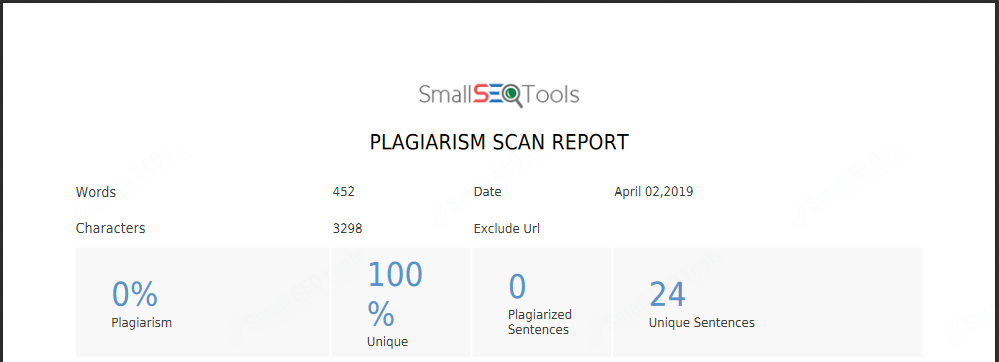
\includegraphics[width=5cm]{figures/5/1174077/teori/plagarismechap5.png}
    \centering
\end{figure}
\end{enumerate}
%%%%%%%%%%%%%%%%%%%%%%%%%%%%%%%%%%%%%%%%%%%%%%%%%%%%%%%%%%%%%%%%%%%%%%%%%%%%%%%%%%%%%%%%%%%%%
\section{Alfadian Owen}
\subsection{Soal 1}
 fungsi device manager di windows dan folder dev di linux.

Device manager digunakan untuk menampilkan seluruh hardware yang bisa di inisialisasi (dikenali) oleh windows.

dev merupakan direktori yang fungsinya untuk menyimpan konfigurasi device atau hardware dari sistem

\subsection{Soal 2}
langkah-langkah instalasi driver dari arduino

\begin{itemize}
	\item Hubungkan port usb Arduino ke port usb pc
	\item Setelah terhubung, di bagian kanan bawah pc anda akan ada notifikasi "installing device driver"
	\item setelah itu akan ada notifikasi gagal menginstall, jangan panik karena memang seperti itu
	\item Buka Device Manager
	\item Di dalam Device Manager cari "unknown device" yang ada di dalam "other device"
	\item Klik kanan lalu update driver software
	\item pilih browse my computer software
	\item cari folder instalan software Arduino yang telah di download
	\item klik next
	\item klik install
	\item selesai
\end{itemize}

\subsection{Soal 3}
cara membaca baudrate dan port

baudrate dan port akan langsung terbaca saat Arduino terpasang ke komputer

\subsection{Soal 4}
sejarah pyserial

Pyserial adalah modul Python API untuk mengakses serial port, Pyserial menyediakan API yang seragam di berbagai sistem operasi termasuk windows,linux,dan BSD

\subsection{Soal 5}
Fungsi yang dipakai dari pyserial

\begin{itemize}
	\item Close()

	untuk menutup port

	\item Write()

	untuk menulis string

	\item Read(byte)

	untuk membaca per byte

	\item Readline()

	untuk membaca sampai line terakhir

	\item Serial()

	untuk membuka port

\end{itemize}
\subsection{Soal 6}
Jelaskan kenapa butuh perulangan dan tidak butuh perulangan dalam membaca serial

Perulangan digunakan untuk membaca data tidak hanya satu kali, dengan adanya perulangan kita dapat membaca data berulang kali. Sehingga data yang dibaca dapat muncul berulang kali.

\subsection{Soal 7}
cara membuat fungsi pyserial

Buat definisi seperti di python dengan menulus “def namafungsi() :”


%%%%%%%%%%%%%%%%%%%%%%%%%%%%%%%%%%%%%%%%%%%%%%%%%%%%%%%%%%%%%%%%%%%%%%%%%%%%%%%%%%%%%%%%%%%%%%%%%%%

\section{Fernando Lorencius S/1174072}
	\subsection{Soal 1} 
		\begin{itemize}
			\item Device Manager : Device Manager menampilkan seluruh hardware yang terinstall dalam komputer atau dikenali oleh Windows.

			\item folder /dev : Dalam sistem operasi Linux, device atau perangkat yang tehubung akan dianggap file.dalam folder /dev terdapat file - file  tersebut berada.
		\end{itemize}

	\subsection{Soal 2}
	Langkah - langkah instalasi driver arduino :
		\begin{enumerate}
			\item sambungkan board Arduino yang dimiliki  ke port USB pada komputer atau laptop, setelah melakukan hal tersebut tunggu hingga Windows mencoba untuk menginstall driver sendiri
			\item setelah melakukan step pertama kita harus memiliki dahulu sofware Arduino, file driver arduino terlebih dahulu dan masukkan ke dalam directory yang terdapat pada komputer diusahakan directory di simpan di file yang mudah di cari
		
			
			\item lalu windows akan memberitahukan notifikasi pop up yang menginformasikan bahwa ingin menginstall dirver, namun nanti biasanya tidak akan menemukan drivernya
			
			\item buka Device Manager ,Klik Start – pilih Control Panel. Di dalam Control Panel, pilih System and Security, lalu pilih System. Selanjutnya pilih Device Manager. 
			\item cari unknown device yang terdapat dalam Device Manager.
			
			\item lakukan klik kanan kepada unknown device tersebut ,setelah itu pilih update driver software
		
			
			\item pilih browse my computer for driver software sesuai dengan directory dalam bagian pertama dalam proses instalisasi
			
			
			\item setelah melakukan proses tersebut, klik install dan tunggu hingga proses selesai
			
			
			\item arduino pun sudah bisa di gunakan dalam komputer / laptop  anda 
			
		\end{enumerate}

	\subsection{Soal 3}
	Untuk mengetahui atau membaca baudrate dan port kita diwajibkan menginstall Arduino IDE, setelah melakukan instalasi atau memiliki Arduino IDE  buka menu serial monitor yang terdapat di dalam tab tools. Dari hasil proses tersebut kita dapat melihat baudrate dan port yang sedang terhubung oleh arduin anda.

	\subsection{Soal 4}
PySerial merupakan paket Python yang memberikan akses atau memberikan memfasilitasi komunikasi serial antara Komputer / laptop dengan perangkat keras eksternal. PySerial menyediakan antarmuka untuk berkomunikasi melalui protokol komunikasi serial. Komunikasi serial merupakan protokol komunikasi komputer tertua. PySerial pertama kali diluncurkan pada tahun 2002 dan makin berkembang dalam setiap versinya hingga tahun 2017 lalu.

	\subsection{Soal 5}
		\begin{itemize}
			\item \begin{verbatim} readline()\end{verbatim} : fungsi serial digunakan untuk menerjemahkan sebuah string dari port serial
			\item \begin{verbatim}Serial(sequence)\end{verbatim} :fungsi serial digunakan untuk membuka port serial.
			\item \begin{verbatim}close()\end{verbatim} : fungsi tersebut digunakan untuk menutup port  dan menghentikan pembacaan program
			\item \begin{verbatim}Write()\end{verbatim} : fungsi write menulis data lewat port serial 
			\item \begin{verbatim}read(size)\end{verbatim}	: fungsi read(size) digunakan membaca seluruh jumlah byte dari port serial.
		\end{itemize}

	\subsection{Soal 6}
	Dalam proses membaca serial di Arduino diperlukan perulangan supaya program dapat membaca data secara berulang kali sehingga data yang muncul banyak.Namun apabila tidak dibutuhkan perulangan maka Arduino akan membaca data cukup sekali saja.

	\subsection{Soal 7}
	Untuk membangun fungsi yang menggunakan pyserial hal yang pertama digunakan kita hanya perlu untuk menginisialisasi pembuatan funsi dengan mengunakan perintah fungsi def namafungsi() : lalu masukan indentasi. atau menggunakan fungsi while loop degan menggunakan  fungsi while true:


%%%%%%%%%%%%%%%%%%%%%%%%%%%%%%%%%%%%%%%%%%%%%%%%%%%%%%%%%%%%%%%%%%%%%%%%%%%%%%%%%%%%%%%%%%%%%%%%%%%

\section{Handi Hermawan}
\subsection{Soal Nomor 1}
Apa itu fungsi device manager di windows dan folder /dev di linux?\\
Jawab :
\begin{itemize}
\item Fungsi Device Manager di Sistem Operasi Windows yaitu
\end{itemize}
Beberapa fungsi kegunaan Device Manager yaitu menunjukkan status suatu hardware, menunjukkan informasi detil suatu hardware, mengelola driver hardware, disable  Enable hardware, meng-identifikasi konflik antar hardware dan Device Manager paling sering digunakan untuk pengelolaan driver suatu hardware. 
\begin{itemize}
\item Fungsi Folder /dev di Sistem Operasi Linux
\end{itemize}
Device manager pada linux berada pada folder /dev yang mempunyai arti device. folder ini berisi konfigurasi device pada sistem.

\subsection{Soal Nomor 2}
Jelaskan langkah-langkah instalasi driver dari arduino!\\
Jawab :
\begin{enumerate}
\item Pertama, Download dan Extract Software Arduino IDE
\item Hubungkan Port USB Arduino UNO ke Port USB PC.
\item Maka PC akan mendeteksi keberadaan perangkat baru.
\item Buka Device Manager dengan mengetik Device Manager di Search Program and Files
\item Setelah Device Manager terbuka, silahkan cari “Unknown Device” yang berada di Other Device.
\item Lalu klik kanan pada Unknown device, pilih Update Driver Software.
\item Pilih Browse my computer for driver software, lalu cari Folder Instalan Software Arduino IDE
\item lalu kilik Next, dan Windowspun akan mencari dan menginstal driver yang berada pada Folder tersebut.
\item Setelah muncul peringatan, klik Install.
\item Selesai, Arduino UNO sudah dikenali oleh PC.
\end{enumerate}

\subsection{Soal Nomor 3}
Jelaskan bagaimana cara membaca baud rate dan port dari komputer yang sudah
terinstall driver! \\
Jawab :\\
Cara membaca baudrate dan port kita hanya perlu menginstall Arduino IDE, setelah itu buka menu serial monitor yang berada di tab tools. Dari sana akan terlihat baudrate dan port yang sedang digunakan oleh arduino.

\subsection{Soal Nomor 4}
Jelaskan sejarah library pyserial!
Jawab : \\
Pyserial akses untuk port serial. Ini menyediakan backends untuk Python berjalan pada Windows, OSX, Linux, BSD (mungkin sistem yang mendukung POSIX) dan IronPython. Modul bernama "serial" secara otomatis memilih backend yang sesuai. PySerial pertama kali diluncurkan pada tahun 2002 yang makin berkembang dalam setiap versinya hingga tahun 2017 lalu.

\subsection{Soal Nomor 5}
Jelaskan fungsi-fungsi apa saja yang dipakai dari library pyserial!\\
Jawab :\\
\begin{itemize}
\item Serial fungsi ini untuk membuka port serial
\item readline berguna untuk membaca sebuah string dari port serial.
\item read(size) berguna untuk membaca jumlah byte dari port serial.
\item close berguna untuk menutup port serial.
\end{itemize}

\subsection{Soal Nomor 6}
Jelaskan kenapa butuh perulangan dan tidak butuh perulangan dalam membaca serial!\\
Jawab :\\
\begin{itemize}
\item Perulangan
\end{itemize}
Dalam perulangan diperlukan untuk untuk mengulangi perintah agar lebih mudah dan tidak terjadi penumpukan kodingan. Perulangan dijalankan jika kondisi benar dan akan berhenti jika kondisi salah.

\begin{itemize}
\item Tidak butuh perulangan
\end{itemize}
Dan apabila perintah dijalankan sekali, kita tidak memerlukan perulangan.

\subsection{Soal Nomor 7}
Jelaskan bagaimana cara membuat fungsi yang menggunakan pyserial!\\
Jawab :\\
Cara membuat fungsi sama seperti pembuatan fungsi seperti biasa namun method dari pyserial dimasukkan kedalam fungsi dan dipanggil fungsi yang kita buat tadi seperti itulah.

\par Scan Plagiarisme
\begin{figure}[ht!]
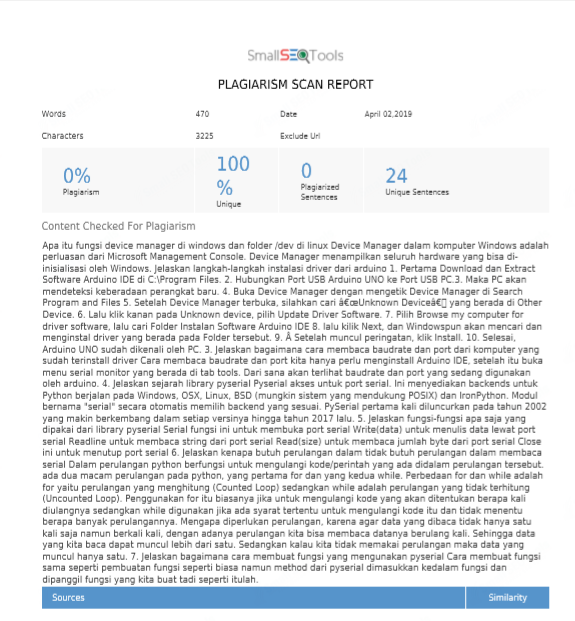
\includegraphics[width=5cm]{figures/5/1174080/Teori/plagiarismteori5.png}
\centering
\caption{plagiarisme}
\end{figure}
%%%%%%%%%%%%%%%%%%%%%%%%%%%%%%%%%%%%%%%%%%%%%%%%%%%%%%%%%%%%%%%%%%%%%%%%%%%%%%%%%%%%%
\section{Muhammad Abdul Gani Wijaya}
{\Large \textbf{Pemahaman Teori}}
\subsection{No. 1}
Device Manager yang ada pada Windows, adalah perluasan dari Microsoft Management Console. Device Manager dapat menampilkan dan mengelola seluruh hardware yang bisa di-inisialisasi (dikenali) oleh Windows. Tampilannya Device Manager telah dikelompokkan sedemikian rupa sehingga akan memudahkan pengelolaan setiap hardware yang ada. Device Manager sangat membantu dalam mengelola (manage) semua hardware yang terpasang dan terdeteksi di dalam Windows. Pada hardware seperti harddisk, kartu VGA, sound, keyboard, perangkat USB dll. akan mudah untuk dikonfigurasi oleh Device Manager ini.
/dev/ : adalah direktori yang berfungsi untuk menyimpan konfigurasi device atau hardware dari system pada linux, seperti harddisk (hda, sda), terminal (tty) etc.

/dev/ : adalah direktori yang berfungsi untuk menyimpan konfigurasi device atau hardware dari system pada linux, seperti harddisk (hda, sda), terminal (tty) etc.

\subsection{No. 2}
Jelaskan langkah-langkah instalasi driver dari arduino!

\hfill \break
Berikut ini adalah langkah-langkah instalasi driver dari Arduino UNO di Windows:

\begin{enumerate}
    \item Pertama double click pada Installer Arduino
    \item Lalu akan muncul License Agreement, klik I Agree
    \begin{figure}[H]
		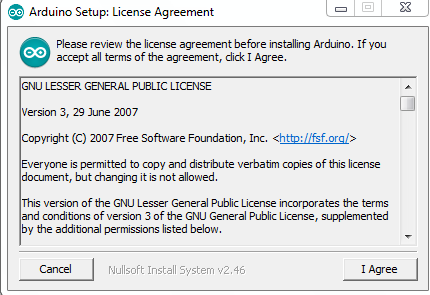
\includegraphics[width=10cm]{figures/5/1174071/Teori/1.png}
		\centering
	\end{figure}
    \item Lalu akan diminta menetukan lokasi instalasi Arduino.
    Anda bisa mengubahnya sesuai keinginan atau membiarkannya tetap default.
    \begin{figure}[H]
		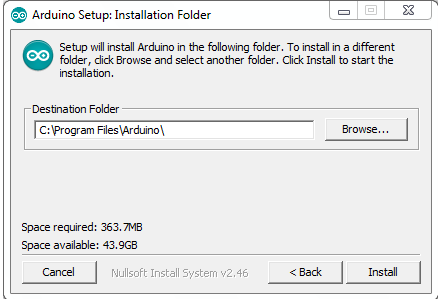
\includegraphics[width=10cm]{figures/5/1174071/Teori/2.png}
		\centering
	\end{figure}
    \item Setelah akan ditampilkan jendela Installation Options. Centang saja semuanya lalu klik next.
    \begin{figure}[H]
		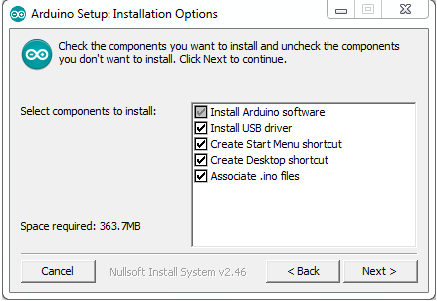
\includegraphics[width=10cm]{figures/5/1174071/Teori/3.png}
		\centering
	\end{figure}
    \item Lalu proses instalasi seperti pada gambar berikut.
    \begin{figure}[H]
		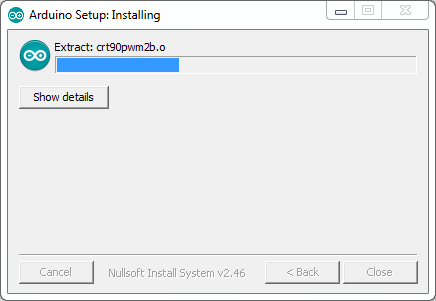
\includegraphics[width=10cm]{figures/5/1174071/Teori/4.png}
		\centering
	\end{figure}
    \item Ditengan installai muncul Security Warning untuk instalasi Arduino USB driver, klik install.
    \begin{figure}[H]
		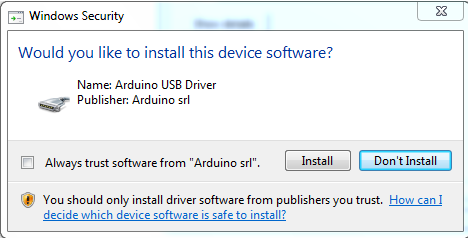
\includegraphics[width=10cm]{figures/5/1174071/Teori/5.png}
		\centering
	\end{figure}
    \item Tunggu sampai installasi complete.
    \begin{figure}[H]
		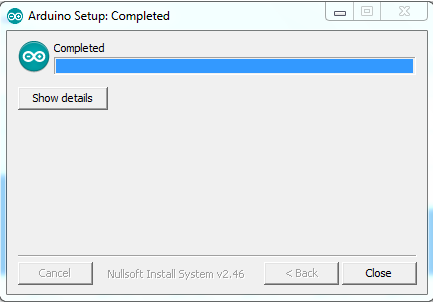
\includegraphics[width=10cm]{figures/5/1174071/Teori/6.png}
		\centering
	\end{figure}
    \item Instalasi Ardunio selesai, dan Arduino Driver siap digunakan.

\end{enumerate}

\subsection{No. 3}
\begin{enumerate}
    \item Pertama buka Device Manager pada laptop
    \item Kemudian klik Ports (COM LPT)
    \item Klik pada Arduino yang terhubung
    \item Klik di tab Port Setting
    \item Di Port Setting ditampilkan Bit Per Second
\end{enumerate}

\subsection{No. 4}
PySerial adalah paket dari Python yang menfasilitasi komunikasi serial antara PC dengan perangkat keras eksternal. PySerial menyediakan antarmuka untuk berkomunikasi melalui protokol komunikasi serial. Komunikasi serial adalah salah satu protokol komunikasi komputer tertua. Protokol komunikasi serial digunakan sebelum adanya USB yang digunakan oleh komputer dan perangkat keras lain seperti mouse, keyboard, dan webcam.

\subsection{Soal No. 5}
\begin{enumerate}
	\item Serial 		: Membuka port serial
	\item Write 		: Menulis data dengan port serial
	\item Readline  	: Membaca port serial
	\item Read	    	: Membaca jumlah byte pada port serial.
	\item Close	    	: Menutup port serial

\end{enumerate}

\subsection{No. 6}
Perulangan diperlukan untuk membaca data berulang terus-menerus untuk menampilkan banyak data. Jika tidak menggunakan perulangan Arduino hanya dapat membaca data satu kali. 

\subsection{No. 7}
Seperti python pada umumnya, fungsi nya dibuat dengan mendeklarasikan def lalu nama fungsinya lalu diikuti dengan isi pada fungsi tersebut.

\subsection{Cek Plagiarisme}
\begin{figure}[H]
		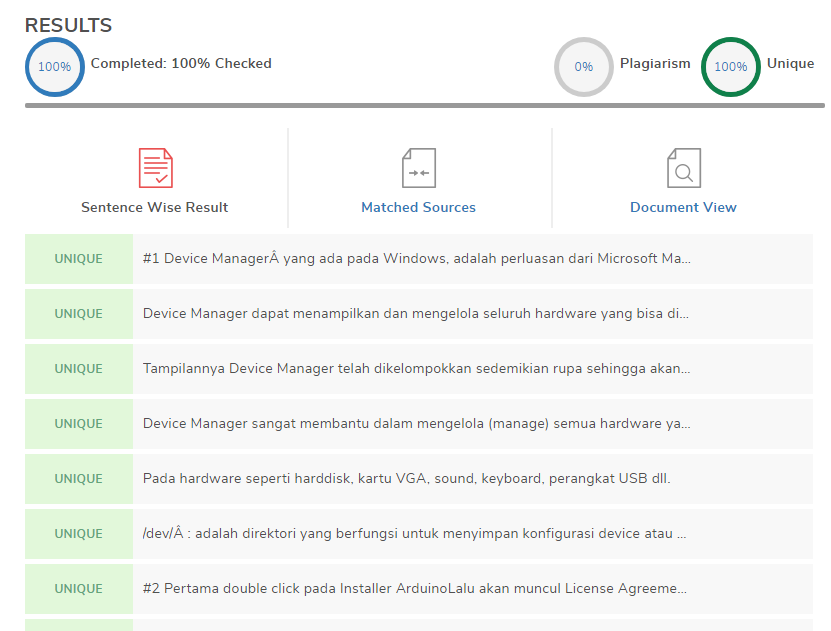
\includegraphics[width=10cm]{figures/5/1174071/Teori/plagiarisme.png}
		\centering
	\end{figure}
%%%%%%%%%%%%%%%%%%%%%%%%%%%%%%%%%%%%%%%%%%%%%%%%%%%%%%%%%%%%%%%%%%%%%%%%%%%%%%%%%%%%%%%%%%
%PRAKTEK
%\chapter{Praktek Komunikasi Perangkat keras}
%\section{Ainul Filiani}
\subsection{Praktek}
\subsubsection{Buatlah fungsi (file terpisah/library dengan nama NPM realtime.py) untuk mendapatkan data langsung dari arduino}
\lstinputlisting[firstline=8, lastline=14]{src/5/1174073/praktek/1174073_realtime.py}

\subsubsection{Buatlah fungsi (file terpisah/library dengan nama NPM save.py) untuk mendapatkan data langsung dari arduino dengan looping}
\lstinputlisting[firstline=8, lastline=15]{src/5/1174073/praktek/1174073_save.py}

\subsubsection{Buatlah fungsi (file terpisah/library dengan nama NPM realtime.py) untuk mendapatkan data dari arduino dan langsung ditulis kedalam file csv}
\lstinputlisting[firstline=16, lastline=29]{src/5/1174073/praktek/1174073_realtime.py}

\subsubsection{Buatlah fungsi (file terpisah/library dengan nama NPM csv.py) untuk membaca file csv hasil arduino dan mengembalikan ke fungsi}
\lstinputlisting[firstline=9, lastline=17]{src/5/1174073/praktek/1174073_csv.py}

\subsubsection{Penanganan Error}
Untuk kali ini saya menemukan Type Error, yaitu error yang menampilkan jika type data na berbeda berusaha disatukan.
\lstinputlisting[firstline=8, lastline=18]{src/5/1174073/praktek/1174073.py}
%%%%%%%%%%%%%%%%%%%%%%%%%%%%%%%%%%%%%%%%%%%%%%%%%%%%%%%%%%%%%%%%%%%%%%%%%%%%%%%%%%%%%

\section{Alfadian Owen}
\subsection{Soal 1}
Buatlah fungsi untuk mendapatkan data langsung dari arduino
\lstinputlisting[firstline=7, lastline=14]{src/5/1174091/Praktek/1174091_realtime.py}

\subsection{Soal 2}
Buatlah fungsi untuk mendapatkan data langsung dari arduino dengan looping
\lstinputlisting[firstline=7, lastline=15]{src/5/1174091/Praktek/1174091_save.py}

\subsection{soal 3}
Buatlah fungsi untuk mendapatkan data dari arduino dan langsung ditulis kedalam file csv
\lstinputlisting[firstline=16, lastline=25]{src/5/1174091/Praktek/1174091_realtime.py}

\subsection{Soal 4}
Buatlah fungsi untuk membaca file csv hasil arduino dan mengembalikan ke fungsi
\lstinputlisting[firstline=7, lastline=15]{src/5/1174091/Praktek/1174091_csv.py}

\subsection{Penanganan Error}
Buatlah fungsi untuk membaca file csv hasil arduino dan mengembalikan ke fungsi
\lstinputlisting[firstline=7, lastline=15]{src/5/1174091/Praktek/1174091_error.py}

%%%%%%%%%%%%%%%%%%%%%%%%%%%%%%%%%%%%%%%%%%%%%%%%%%%%%%%%%%%%%%%%%%%%%%%%%%%%%%%%%%%%%%%%%%%%%%%
\section{Alvan Alvanzah/1174077}
\subsection{Ketrampilan Pemrograman}
\begin{enumerate}
    \item Buatlah  fungsi  (file  terpisah/library  dengan  nama  NPMrealtime.py)  untuk mendapatkan data langsung dari arduino.
    \lstinputlisting[firstline=1, lastline=7]{src/5/1174077/praktek/1174077_realtime.py}
    
    \item Buatlah fungsi (file terpisah/library dengan nama NPMsave.py) untuk mendapatkan data langsung dari arduino dengan looping.
    \lstinputlisting[firstline=1, 
    lastline=8]{src/5/1174077/praktek/1174077_save.py}
    
    \item Buatlah  fungsi  (file  terpisah/library  dengan  nama  NPMrealtime.py)  untuk mendapatkan data dari arduino dan langsung ditulis kedalam file csv.
    \lstinputlisting[firstline=9, lastline=23]{src/5/1174077/praktek/1174077_realtime.py}
    
    \item Buatlah fungsi (file terpisah/library dengan nama NPMcsv.py) untuk membaca file csv hasil arduino dan mengembalikan ke fungsi.
    \lstinputlisting[firstline=1, 
    lastline=9]{src/5/1174077/praktek/1174077_csv.py}
    \par Cek Plagiat Praktek
    \begin{figure}[!h]
	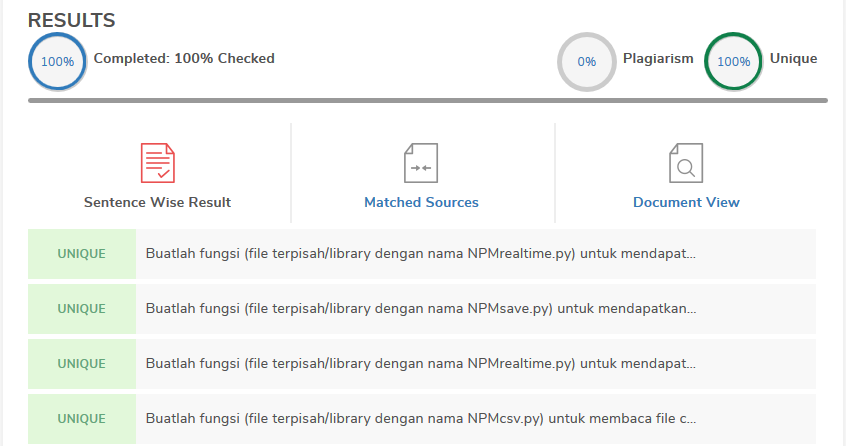
\includegraphics[width=10cm]{figures/5/1174077/praktek/cekpraktek.png}
	\centering
    \end{figure}
\end{enumerate}
\subsection{Ketrampilan Penanganan Error}
\begin{enumerate}
    \item Tuliskan  peringatan  error  yang  didapat  dari  mengerjakan  praktek ketiga  ini, dan  jelaskan  cara  penanganan  error  tersebut.   dan  Buatlah  satu fungsi  yang menggunakan try except untuk menanggulangi error tersebut.
\begin{itemize}
	\item Syntax Errors
	Syntax Errors adalah suatu keadaan saat kode python mengalami kesalahan penulisan. Solusinya adalah memperbaiki penulisan kode yang salah.
	
	\item Name Error
	NameError adalah exception yang terjadi saat kode melakukan eksekusi terhadap local name atau global name yang tidak terdefinisi. Solusinya adalah memastikan variabel atau function yang dipanggil ada atau tidak salah ketik.
	
	\item Type Error
	TypeError adalah exception yang akan terjadi apabila pada saat dilakukannya eksekusi terhadap suatu operasi atau fungsi dengan type object yang tidak sesuai. Solusi dari error ini adalah mengkoversi varibelnya sesuai dengan tipe data yang akan digunakan.
\end{itemize}
\par Fungsi yang menggunakan try except untuk menanggulangi error.
\lstinputlisting[firstline=1, 
lastline=16]{src/5/1174077/praktek/1174077.py}
\end{enumerate}
%%%%%%%%%%%%%%%%%%%%%%%%%%%%%%%%%%%%%%%%%%%%%%%%%%%%%%%%%%%%%%%%%%%%%%%%%%%%%%%%%%%%%%%%%%%%%%%%%%%%%%
\section{Muhammad Abdul Gani Wijaya}
{\Large \textbf{Ketrampilan Pemrograman}}
\subsection{No. 1}
Buatlah  fungsi  (file  terpisah/library  dengan  nama  NPMrealtime.py)  untuk mendapatkan data langsung dari arduino!

\lstinputlisting[firstline=8,lastline=14]{src/5/1174071/Praktek/1174071_realtime.py}


\subsection{No. 2}
Buatlah fungsi (file terpisah/library dengan nama NPMsave.py) untuk mendapatkan data langsung dari arduino dengan looping!

\lstinputlisting[firstline=8,lastline=15]{src/5/1174071/Praktek/1174071_save.py}

\subsection{No. 3}
Buatlah  fungsi  (file  terpisah/library  dengan  nama  NPMrealtime.py) untuk mendapatkan data dari arduino dan langsung ditulis kedalam file csv!

\lstinputlisting[firstline=16,lastline=30]{src/5/1174071/Praktek/1174071_realtime.py}

\subsection{Soal No. 4}
Buatlah fungsi (file terpisah/library dengan nama NPMcsv.py) untuk membaca file csv hasil arduino dan mengembalikan ke fungsi!

\lstinputlisting[firstline=9,lastline=17]{src/5/1174071/Praktek/1174071_csv.py}

\subsection{Keterampilan Penanganan Error}
Tuliskan  peringatan  error  yang  didapat  dari  mengerjakan  praktek  kelima  ini, dan  jelaskan  cara  penanganan  error  tersebut.   dan  Buatlah  satu  fungsi  yang menggunakan try except untuk menanggulangi error tersebut.

\hfill \break
Peringatan errror:
\begin{itemize}
	\item Syntax Errors
	Syntax Errors adalah suatu keadaan saat kode python mengalami kesalahan penulisan. Solusinya adalah memperbaiki penulisan kode yang salah.
	
	\item Name Error
	NameError adalah exception yang terjadi saat kode melakukan eksekusi terhadap local name atau global name yang tidak terdefinisi. Solusinya adalah memastikan variabel atau function yang dipanggil ada atau tidak salah ketik.
	
	\item Type Error
	TypeError adalah exception yang akan terjadi apabila pada saat dilakukannya eksekusi terhadap suatu operasi atau fungsi dengan type object yang tidak sesuai. Solusi dari error ini adalah mengkoversi varibelnya sesuai dengan tipe data yang akan digunakan.
\end{itemize}

\hfill \break
Fungsi untuk menanggulangi error

\lstinputlisting[firstline=9,lastline=24]{src/5/1174071/Praktek/1174071_error.py}
%%%%%%%%%%%%%%%%%%%%%%%%%%%%%%%%%%%%%%%%%%%%%%%%%%%%%%%%%%%%%%%%%%%%%%%%%%%%%%%%%%%%%%%%%%%%%%%

\section{Handi Hermawan-1174080}
\textbf{Ketrampilan Pemrograman}

\subsection{Jawaban Soal No. 1}
\lstinputlisting[caption = Soal no.1, firstline=1, lastline=48]{src/5/1174080/Praktek/1174080_realtime.py}
\subsection{Jawaban Soal No. 2}
\lstinputlisting[caption = Soal no.2, firstline=1, lastline=22]{src/5/1174080/Praktek/1174080_save.py}
\subsection{Jawaban Soal No. 3}
\lstinputlisting[caption = Soal no.3, firstline=25, lastline=47]{src/5/1174080/Praktek/1174080_realtime.py}
\subsection{Jawaban Soal No. 4}
\lstinputlisting[caption = Soal no.4, firstline=1, lastline=9]{src/5/1174080/Praktek/1174080_csv.py}
\subsection{Kode Program Mindwave.py}
\hfill \break
{\Large \textbf{Ketrampilan Penanganan Error}}
\subsection{Jawaban Soal No. 1}
\hfill \break
Peringatan error di praktek kelima ini, yaitu:
\begin{itemize}
	\item Syntax Errors
	Syntax Errors adalah suatu keadaan dimana saat kode python mengalami kesalahan penulisan. Solusinya adalah dengan memperbaiki penulisan kode yang salah.
	\item Name Error
	NameError adalah exception yang terjadi pada saat kode melakukan eksekusi terhadap suatu local name atau global name yang tidak terdefinisi. Solusinya adalah dengan memastikan variabel atau function yang dipanggil ada atau tidak salah ketik.
	\item Type Error
	TypeError adalah exception yang akan terjadi apabila pada saat melakukan eksekusi terhadap suatu operasi atau fungsi dengan type object yang tidak sesuai. Solusi dari error tersebut adalah dengan mengkoversi variabelnya sesuai dengan tipe data yang akan digunakan.
\end{itemize}
\hfill \break
Fungsi yang menggunakan try except untuk menanggulangi error.
\lstinputlisting[caption = Fungsi untuk menanggulangi error menggunakan Try Except, firstline=1, lastline=17]{src/5/1174080/Praktek/1174080_error.py}

%%%%%%%%%%%%%%%%%%%%%%%%%%%%%%%%%%%%%%%%%%%%%%%%%%%%%%%%%%%%%%%%%%%%%%%%%%%%%%%%%%%%%%%%%%%%%%%
\section{Fernando Lorencius S}
\subsection{Soal 1}
Buatlah fungsi (file terpisah/library dengan nama NPM realtime.py) untuk mendapatkan data langsung dari arduino
\lstinputlisting[firstline=8, lastline=17]{src/5/1174072/Praktek/1174072_realtime.py}


\subsection{Soal 2}
Buatlah fungsi (file terpisah/library dengan nama NPM save.py) untuk mendapatkan data langsung dari arduino dengan looping
\lstinputlisting[firstline=10, lastline=15]{src/5/1174072/Praktek/1174072_save.py}


\subsection{Soal 3}
Buatlah fungsi (file terpisah/library dengan nama NPM realtime.py) untuk mendapatkan data dari arduino dan langsung ditulis kedalam file csv
\lstinputlisting[caption="Kode python",firstline=19, lastline=31]{src/5/1174072/Praktek/1174072_realtime.py}
\lstinputlisting[caption="Data yang telah ditulis ke file csv",firstline=0, lastline=24]{src/5/1174072/Praktek/1174072.csv}

\subsection{Soal 4}
Buatlah fungsi (file terpisah/library dengan nama NPM csv.py) untuk membaca file csv hasil arduino dan mengembalikan ke fungsi
\lstinputlisting[firstline=8, lastline=14]{src/5/1174072/Praktek/1174072_csv.py}

\subsection{Ketrampilan Penanganan Error}
Tuliskan peringatan error yang didapat dari mengerjakan praktek ketiga ini, dan jelaskan cara penanganan error tersebut. dan Buatlah satu fungsi yang menggunakan gunakan try except untuk menanggulangi error tersebut.
\begin{itemize}
\item Syntax Errors

Syntax Errors adalah kesalahan pada penulisan syntax atau kode. Solusinya adalah memperbaiki penulisan syntax atau kode

\item Zero Division Error

ZeroDivisonError adalah exceptions yang terjadi saat eksekusi program menghasilkan perhitungan matematika pembagian dengan angka nol (0). Solusinya adalah tidak membagi suatu yang hasilnya nol.

\item Name Error

NameError adalah exception saat kode melakukan eksekusi terhadap local name atau global name yang tidak terdefinisi atau tidak ada. Solusinya adalah memastikan variabel atau function yang akan dipanggil ada didalam program atau tidak salah mengetikannya.

\item Type Error

TypeError adalah exception saat melakukan eksekusi terhadap suatu operasi atau fungsi dengan type object yang tidak sesuai. Solusinya adalah mengkoversi varibelnya sesuai dengan tipe data sesuai dengan yang akan digunakan.

\end{itemize}
\lstinputlisting[firstline=8, lastline=23]{src/5/1174072/Praktek/1174072_error.py}





%%%%%%%%%%%%%%%%%%%%%%%%%%%%%%%%%%%%%%%%%%%%%%%%%%%%%%%%%%%%%%%%%%%%%%%%%%%%%%%%%%%%%%%%%%%%%%%

\chapter{tugas 6}
\section{Ainul Filiani}
\begin{enumerate}
\item Apa itu fungsi library matplotlip ?

Data yang kita olah tentu tidak bagus apabila ditampilkan begitu saja dengan tabel hitam saja kepada investor atau manajemen. Bila ditampilkan dengan sejumlah grafik berwarna pasti akan terlihat lebih menarik ketika melihatnya. Matplotlib membantu kita untuk memvisualisasikan data dengan lebih indah dan rapi.
Ada plot untuk menampilkan data dengan cara 2D atau 3D. Sehingga kita dapat menampilkan data yang telah kita olah sesuai kebutuhan. Matplotlib pun terintegrasi dengan iPython Notebook atau Jupyter dimana kita dapat membuat sebuah buku interaktif yang dapat diberi penjelasan dan kode yang disisipkan begitupun hasil plottingnya.
Matplotlib adalah library paling banyak atau sering digunakan oleh data science untuk menyajikan datanya ke dalam visual yang lebih baik.

\item jelaskan langkah-langkah membuat sumbu X dan Y di matplotlip?

untuk membuat sumbu x dan y kita bisa menggunakan list untuk mempermudah penyimpanan nilai setiap sumbunya.
contoh pembuatannya: 
\lstinputlisting[firstline=9, lastline=10]{src/6/1174073/teori/1174073.py}

\item jelaskan bagaimana perbedaan fungsi dan cara pakai untuk berbagai jenis (bar, histogram, dll). jenis plot di matplotlip ?  

Untuk perbedaan fungsi plot yang digunakan adalah bentuk bentuk grafik yang akan di tampilkan sesuai dengan perintah yang digunakan pada pemogramannya.
Dan untuk cara pengguna plot tersebut sebagai berikut
\begin{itemize}
    \item line
    Perintah yang digunakan untuk membuat grafik line sebagai berikut.
    \lstinputlisting[firstline=12, lastline=14]{src/6/1174073/teori/1174073.py}
    \item bar
    Dalam Penggunaan plot bar koordinat x nya itu yang awal, dan untuk Y nya adalah yang kedua
    \lstinputlisting[firstline=16, lastline=25]{src/6/1174073/teori/1174073.py}
    \item histogram
    Dalam penggunaan plot histogram titik x nya bisa tidak sama dengan titik Y.
    untuk penggunaannya bisa sebagai berikut.
    \lstinputlisting[firstline=27, lastline=34]{src/6/1174073/teori/1174073.py}
    \item scatter
    Untuk penggunaa plot scatter atau bisa juga d bilang diagram titik.
    Contoh dari penggunaannya bisa dilihat sebagai berikut.
    \lstinputlisting[firstline=36, lastline=49]{src/6/1174073/teori/1174073.py}
    \item Stack plot
    Untuk penggunaan stack plot ini seperti diagram line, tapi ada fill colornya,jadi antar line itu bisa berdekatan.
    Berikut Contoh penggunaannya
    \lstinputlisting[firstline=82, lastline=92]{src/6/1174073/teori/1174073.py}
\end{itemize} 

\item Jelaskan bagaimana cara menggunakan legend dan lebel serta kaitannya dengan fungsi tersebut 

Untuk menggunakan legend dan label bisa di lihat dibawah ini
\lstinputlisting[firstline=20, lastline=22]{src/6/1174073/teori/1174073.py}
penggunaan legend itu untuk mempermudahkita dalam membaca grafik, legend itu sendiri berisi info info dari grafik yang ada seperti nama, kemudian bentuk dan warna.
kemudian untuk label itu sendiri digunakan untuk membedakan nama titik X dan titik Y.

\item Jelaskan apa fungsi dari subplot di matplotlib dan agaimana cara kerja dari fungsi subplot, sertakan ilustraasi dan gambar sendiri dan apa parameternya jika ingin menggambar plot dengan 9 subplot didalamnya ? 

fungsi dari subplot dari matplotlib untuk bisa membuat lebih dari 1 grafik dalam sebuah program.
untuk cara kerjanya sendiri bisa d cek sebagai berikut
\lstinputlisting[firstline=94, lastline=104]{src/6/1174073/teori/1174073.py}
untuk parameternya sendiri saya menggunakan x dan y x sebagai koordinat x dan y sebagai koordinat y.
\begin{figure}[H]	
    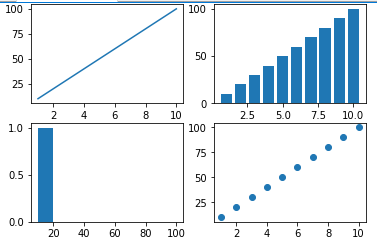
\includegraphics[width=5cm]{figures/6/1174073/teori/satu.png}
    \centering
    \caption{SubPlot}
\end{figure}

\item sebutkan semua pparameter color yang bisa digunakan contoh: m,c,r,k,...

Untuk parameter color yang bisa digunakan terdiri dari 2 type warna.

Tipe Warna RGB

Untuk keterangannya sebagai berikut
\begin{enumerate}
\item R untuk warna Red atau Merah
\item G untuk warna Green atau Hijau
\item B untuk warna Blue atau Biru
\end{enumerate}
Tipe warna CMYK

Untuk keterangannya sebagai berikut
\begin{enumerate}
\item    C untuk warna Cyan atau Biru Muda
\item    M untuk warna Mangenta atau Merah Tua
\item    Y untuk warna Yellow Atau Kuning
 \item   K untuk warna blacK atau Hitam
\end{enumerate}

\item Jelaskan bagaimana cara kerja dari fungsi hist, sertakan ilustrasi dan gambar sendiri?

Untuk fungsi histogram ini kedua titik koordinat boleh tidak sama. Misalnya x nya ada 10 nilai sedangkan Y nya ada 5 nilai, itu tidak akan jadi masalah karena diagram ini digunakan untuk mendata usia dari rentang tertentu atau kebutuhan lainnya.
Ini merupakan contoh dari penggunaan histogram
\lstinputlisting[firstline=27, lastline=34]{src/6/1174073/teori/1174073.py}
dan ini merupakan grafik histogram tersebut.
\begin{figure}[H]	
    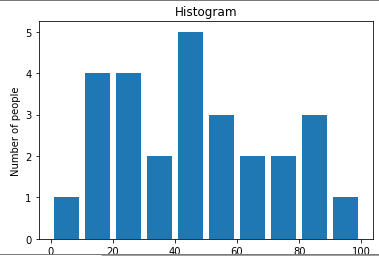
\includegraphics[width=5cm]{figures/6/1174073/teori/histogram.png}
    \centering
    \caption{Diagram Histogram}
\end{figure}

\item jelaskan lebih mendalam tentang parameter dari fungsi pie diantaranya labels, colors,startangle, shadow, explode, autopct.

Berikut penjelasan tentang parameter yang ada dalam pie chart
\begin{itemize}
    \item label
    Label digunakan untuk mempermudah pembaca dalam membaca diagram pie
    \item color
    warna digunakan untuk membedakan antar data
    \item startangle
    Digunakan untuk sudut yang digunakan untuk memulai diagram pie tersebut
    \item shadow
    bayangan digunakan untuk membuat bayangan dari setiap diagram pie yang menonjol
    \item explode
    explode digunakan untuk mengeluarkan suatu data agar data tersebut terlihat menonjol
    \item autopct
    Digunakan sesuai dengan berapa angka dibelakang koma yang kita inginkan
\end{itemize} 
\end{enumerate}
%%%%%%%%%%%%%%%%%%%%%%%%%%%%%%%%%%%%%%%%%%%%%%%%%%%%%%%%%%%%%%%
\section{Sekar Jasminei}
\begin{enumerate}

\item 1. Apa itu fungsi library Matplotlib
Matplotlib adalah sebuah library pada python yang digunakan untuk membuat diagram. Library ini biasanya menghasilkan ploting 2D.\\

Ada plot untuk menampilkan data secara 2D atau 3D. sehingga kamu dapat menampilkan data yang telah kamu olah sesuai kebutuhan. Matplotlib pun terintegrasi dengan ipython notebook atau jupyter dimana kamu dapat membuat sebuah buku interaktif yang dapat diberi penjelasan dan kode yang disisipkan begitupun hasil plottingnya.\\

\item 2. Jelaskan langkah-langkah membuat sumbu X dan Y di matplotlib.
untuk membuat sumbu x dan y kita bisa membuatnya menggunakan list untuk mempermudah penyimpanan nilai setiap sumbunya.\\
\lstinputlisting[firstline=9, lastline=11]{src/6/1174075/teori/1174075.py}

\item 3. Jelaskan bagaimana perbedaan fungsi dan cara pakai untuk berbagai jenis(bar,histogram,scatter.dll) jenis plot di matloptlib
Untuk perbedaan fungsi plot yang digunakan adalah bentuk bentuk grafik yang akan di tampilkan sesuai dengan perintah yang digunakan pada pemogramannya.\\

line itu untuk perintah yang digunakan untuk membuat grafik line sebagai berikut.\\
\lstinputlisting[firstline=12, lastline=15]{src/6/1174075/teori/1174075.py}
Bar itu di dalam Penggunaan plot bar koordinat x nya itu yang awal, dan untuk Y nya adalah yang kedua.\\
\lstinputlisting[firstline=16, lastline=26]{src/6/1174075/teori/1174075.py}
Histrogram itu di dalam penggunaan plot histogram titik x nya bisa tidak sama dengan titik Y. untuk penggunaannya bisa sebagai berikut.\\
\lstinputlisting[firstline=27, lastline=35]{src/6/1174075/teori/1174075.py}
scatter untuk penggunaa plot scatter atau bisa juga d bilang diagram titik.\\
\lstinputlisting[firstline=36, lastline=50]{src/6/1174075/teori/1174075.py}
Stack plot untuk penggunaan stack plot ini seperti diagram line, tapi ada fill colornya,jadi antar line itu bisa berdekatan.\\
\lstinputlisting[firstline=82, lastline=92]{src/6/1174075/teori/1174075.py}

\item 4. Jelaskan bagaimana cara menggunakan legend dan label serta kaitannya dengan fungsi tersebut.
Contoh source code lengkap disertai dengan link "editor" untuk mencoba (try it) dan melihat hasil (preview) kode.\\

Elemen yang akan ditambahkan ke legenda ditentukan secara otomatis, ketika Anda tidak memberikan argumen tambahan.\\

Garis-garis spesifik dapat dikecualikan dari pemilihan elemen legenda otomatis dengan mendefinisikan label dimulai dengan garis bawah.\\

\item 5. Jelaskan apa fungsi dari subplot di matplotlib dan fungsi dari subplot dari matplotlib untuk bisa membuat lebih dari 1 grafik dalam sebuah program.\\

Misalnya, kita dapat membuat sumbu inset di sudut kanan atas sumbu lain dengan mengatur posisi x dan y ke 0,65 yaitu, mulai dari 65 peren dari lebar dan 65 persen  dari ketinggian gambar dan x dan y meluas ke 0,2 yaitu, ukuran sumbu adalah 20 persen  dari lebar dan 20persen dari tinggi gambar.\\

Simple Grids of Subplots itu kebutuhan yang cukup umum sehingga Matplotlib memiliki beberapa rutinitas kenyamanan yang membuatnya mudah dibuat. Level terendah adalah plt.subplot (), yang membuat subplot tunggal di dalam kisi. Seperti yang Anda lihat, perintah ini membutuhkan tiga argumen bilangan bulat — jumlah baris, jumlah kolom, dan indeks plot yang akan dibuat dalam skema ini, yang berjalan dari kiri atas ke kanan bawah.\\

The Whole Grid in One Go itu  membuat grid besar subplot, terutama jika Anda ingin menyembunyikan label sumbu x dan y pada plot bagian dalam. Untuk tujuan ini, plt.subplots () adalah alat yang lebih mudah digunakan.\\
\lstinputlisting[firstline=94, lastline=104]{src/6/1174075/teori/1174075.py}
 
\item 6. Sebutkan semua parameter color yang bisa digunakan(contoh: m,c,r,k,...dkk)
Tipe Warna RGB
    Untuk keterangannya sebagai berikut
    R untuk warna Red atau Merah
    G untuk warna Green atau Hijau
    B untuk warna Blue atau Biru.\\
    
Tipe warna CMYK
    Untuk keterangannya sebagai berikut
    C untuk warna Cyan atau Biru Muda
    M untuk warna Mangenta atau Merah Tua
    Y untuk warna Yellow Atau Kuning
    K untuk warna blacK atau Hitam.\\

\item 7. Jelaskan bagaimana cara kerja dari fungsi hist , sertakan ilustrasi dan gambar sendiri.
Untuk fungsi histogram ini kedua titik koordinat boleh tidak sama. Misalnya x nya ada 10 nilai sedangkan Y nya ada 5 nilai, itu tidak akan jadi masalah karena diagram ini digunakan untuk mendata usia dari rentang tertentu atau kebutuhan lainnya.\\

Ini merupakan contoh dari penggunaan histogram.\\

\item 8. Jelaskan lebih dalam tentang parameter dari fungsi pie diantaranya labels , color , startangle , shadow , explode , autopct.
Jika jumlah x <1, maka nilai x memberikan area fraksional secara langsung dan array tidak akan dinormalisasi.\\

labels : Label digunakan untuk mempermudah pembaca dalam membaca diagram pie.\\

color : warna digunakan untuk membedakan antar data.\\

startangle : Digunakan untuk sudut yang digunakan untuk memulai diagram pie tersebut.\\

shadow :  bayangan digunakan untuk membuat bayangan dari setiap diagram pie yang menonjol.\\

explode : explode digunakan untuk mengeluarkan suatu data agar data tersebut terlihat menonjol.\\

autopct : Digunakan sesuai dengan berapa angka dibelakang koma yang kita inginkan.\\
\end{enumerate}
%%%%%%%%%%%%%%%%%%%%%%%%%%%%%%%%%%%%%%%%%%%%%%%%%%%%%%%%%%%%%%%%%%%%%%%%%%%%%%%%%%%%%%%%%%%%%%%%%%%

\section{Kaka Kamaludin}
\subsection{Soal 1}
Matplotlib merupakan library python yang berfungsi untuk mengasilkan plot yang di paparkan dengan toolkit GUI yang interaktif.

\subsection{Soal 2}
penulisan Sumbu x dan Y, pada plt.plot(xxx, yyy) diwali dengan sumbu x lalu y.
\lstinputlisting[firstline=1, lastline=13]{src/6/1174067/Teori/1174067_teori.py}


\subsection{Soal 3}
\begin{itemize}
	\item Line Plot, berfungsi untuk menamplikan data yang berkelanjutan dalam priode tertentu.
	\lstinputlisting[firstline=15, lastline=18]{src/6/1174067/Teori/1174067_teori.py}
	
	\item Pie Chart, berfungsi untuk menamplikan bagian suatu data terhadap jumlah keseluruhan secara proporsional. 	setiap bagian data dihitung dalam persentase. pie chart berbentuk bulat seperti potongan kue.
	\lstinputlisting[firstline=20, lastline=42]{src/6/1174067/Teori/1174067_teori.py}
	
	\item Bar Chart, berfungsi sebagai perbandingan beberapa kategori data, ditampilkan dalam bentuk batang.
	\lstinputlisting[firstline=43, lastline=53]{src/6/1174067/Teori/1174067_teori.py}
	
	\item Scatter Chart, biasa digunakan untuk pengujian pola hubungan antara dua variable.
	\lstinputlisting[firstline=54, lastline=69]{src/6/1174067/Teori/1174067_teori.py}
	
	\item Histogram Chart, berfungsi untuk perbandingan data dalam bentuk range.
	\lstinputlisting[firstline=70, lastline=79]{src/6/1174067/Teori/1174067_teori.py}
	
	\item Stack Chart,.
	\lstinputlisting[firstline=80, lastline=101]{src/6/1174067/Teori/1174067_teori.py}		
\end{itemize}

\subsection{Soal 4}
Legend dan Label berfungsi untuk mempermudah dalam pembacaan chart tersebut. contohnya:
\lstinputlisting[firstline=102, lastline=119]{src/6/1174067/Teori/1174067_teori.py}

\subsection{Soal 5}
sublpot berfungsi untuk membuat plot lebih dari 1, contoh:
\lstinputlisting[firstline=120, lastline=148]{src/6/1174067/Teori/1174067_teori.py}

\subsection{Soal 6}
parameter color bisa dibuat dengan menggunakan float value(0.1, 0.2, 0.5, 0.3), hex ('\# 0F0F0F' atau '\#0F0F0F0F'), xkcd color ('xkcd:sky blue'), Tableau Colors ('tab:gray')
\begin{itemize}
    \item Tipe Warna RGB

    R untuk warna Red atau Merah,
    G untuk warna Green atau Hijau,
    B untuk warna Blue atau Biru,
    \item Tipe warna CMYK

    C untuk warna Cyan atau Biru Muda,
    M untuk warna Mangenta atau Merah Tua,
    Y untuk warna Yellow Atau Kuning,
    K untuk warna black atau Hitam
\end{itemize}
\lstinputlisting[firstline=149, lastline=169]{src/6/1174067/Teori/1174067_teori.py}

\subsection{Soal 7}
Untuk fungsi histogram ini kedua titik koordinat boleh tidak sama. Misalnya x nya ada 10 nilai sedangkan Y nya ada 5 nilai, itu tidak akan jadi masalah karena diagram ini digunakan untuk mendata usia dari rentang tertentu atau kebutuhan lainnya.
	\lstinputlisting[firstline=170, lastline=177]{src/6/1174067/Teori/1174067_teori.py}

\subsection{Soal 8}
\begin{itemize}
    \item label
    Label digunakan untuk mempermudah pembaca dalam membaca diagram pie
    \item color
    warna digunakan untuk membedakan antar data
    \item startangle
    Digunakan untuk sudut yang digunakan untuk memulai diagram pie tersebut
    \item shadow
    bayangan digunakan untuk membuat bayangan dari setiap diagram pie yang menonjol
    \item explode
    explode digunakan untuk mengeluarkan suatu data agar data tersebut terlihat menonjol
    \item autopct
    Digunakan sesuai dengan berapa angka dibelakang koma yang kita inginkan
\end{itemize}

%%%%%%%%%%%%%%%%%%%%%%%%%%%%%%%%%%%%%%%%%%%%%%%%%%%%%%%%%%%%%%%%%%%%%%%%%%%%%%%%%%%%%%%%%%%%%%%%%%%
\section{Alvan Alvanzah/1174077}
\subsection{Pemahaman Teori}

\begin{enumerate}
    \item Apa itu fungsi library matplotlib
    \par Matplotlib berfungsi untuk memvisualkan data dengan lebih indah dan rapi dengan menampilkan data secara 2D. Matplotlib mencoba membuat hal-hal mudah menjadi mudah dan hal-hal sulit menjadi mungkin. Dengan Matplotlib dapat membuat plot, histograms, power spectra, bar charts, errorcharts, scatterplots, dll.
    
    \item Jelaskan langkah-langkah membuat sumbu X dan Y di matplotlib.
    \begin{itemize}
        \item pertama import library matplotlib.
        \item kedua membuat isi dari variabel sumbu x dan y.
        \item ketiga tampilkan hasil dari sumbu x dan y.
    \end{itemize}
    \lstinputlisting[firstline=8, lastline=13]{src/6/1174077/teori/1174077.py}
    
    \item Jelaskan bagaimana perbedaan fungsi dan cara pakai untuk berbagai jenis (bar, histogram, scatter, line, dll) jenis plot di matplotlib.
    \par Untuk perbedaan fungsi plot yang digunakan adalah bentuk-bentuk grafik yang akan di tampilkan sesuai dengan perintah yang digunakan pada pemogramannya.
    Dan untuk cara pengguna plot tersebut sebagai berikut:
    \begin{itemize}
        \item bar
        
        Dalam Penggunaan plot bar koordinat x nya itu yang awal, dan untuk Y nya adalah yang kedua.
        \lstinputlisting[firstline=15, lastline=25]{src/6/1174077/teori/1174077.py}
        \item histogram
        
        Dalam penggunaan plot histogram titik x nya bisa tidak sama dengan titik Y.
        \lstinputlisting[firstline=28, lastline=36]{src/6/1174077/teori/1174077.py}
        \item scatter
        
        Untuk penggunaa plot scatter atau bisa juga d bilang diagram titik.
        \lstinputlisting[firstline=39, lastline=53]{src/6/1174077/teori/1174077.py}
        \item line
        
        Perintah yang digunakan untuk membuat grafik line sebagai berikut.
        \lstinputlisting[firstline=56, lastline=59]{src/6/1174077/teori/1174077.py}
    \end{itemize}
    
    \item Jelaskan bagaimana cara menggunakan legend dan label serta kaitannya dengan fungsi tersebut.
    \begin{itemize}
        \item Untuk membuat legenda pada plot dapat menggunakan syntax fungsi legend pada MATLAB.
        \lstinputlisting[firstline=21, lastline=21]{src/6/1174077/teori/1174077.py}
        \item Untuk menambah label pada garis sumbu pada grafik dapat menggunakan syntax fungsi xlabel dan fungsi ylabel pada MATLAB.
        \lstinputlisting[firstline=22, lastline=23]{src/6/1174077/teori/1174077.py}
        \par Kaitannya untuk memperjelas informasi dari grafik yang dibuat.
    \end{itemize}
    
    \item Jelaskan apa fungsi dari subplot di matplotlib, dan bagaimana cara kerja dari fungsi subplot, sertakan ilustrasi dan gambar sendiri dan apa parameternya jika ingin menggambar plot dengan 9 subplot di dalamnya.
    \par fungsi dari subplot dari matplotlib untuk bisa membuat lebih dari 1 grafik dalam sebuah program.
    \par untuk cara kerjanya sendiri bisa di cek sebagai berikut:
    \lstinputlisting[firstline=62, lastline=84]{src/6/1174077/teori/1174077.py}
    \par Cara penggunaannya sebagai contoh saya ambil plt.subplot(221), pada angka 2 yang pertama adalah pembagian keatas kalo kita mau bagi 3 keatas kita isi angka pertama dengan 3, angka 2 yang kedua adalah pembagian kesamping penggunaannya sama kaya angka pertama kalo kita mau ngebagi kesamping 4 kita isi angka kedua 4, dan angka 1 pada angka ketiga itu tempat disimpannya grafik yang akan dimunculkan
    
    \item Sebutkan semua parameter color yang bisa digunakan (contoh:  m,c,r,k,...  dkk)
    Parameter warna yang bisa digunakan dibagi menjadi 2 tipe:
    \begin{itemize}
	    \item RGB
	
	Untuk keterangannya sebagai berikut
    R untuk warna Red atau Merah
    G untuk warna Green atau Hijau
    B untuk warna Blue atau Biru
    
        \item CMYK
    
    Untuk keterangannya sebagai berikut
    C untuk warna Cyan atau Biru Muda
    M untuk warna Mangenta atau Merah Tua
    Y untuk warna Yellow Atau Kuning
    K untuk warna Black atau Hitam
    \end{itemize}
    
    \item Jelaskan bagaimana cara kerja dari fungsi hist, sertakan ilustrasi dan gambar sendiri.
    \par Untuk histogram kita tidak boleh memiliki isi variable x dan y yang sama. Misal x-nya ada 10 nilai sedangkan Y-nya ada 5 nilai, data tersebut tidak menjadi masalah karena pada histogram data yang dimunculkan adalah data rentang dari data variable y. Dan ini adalah contoh dari penggunaan histogram.
    \lstinputlisting[firstline=87, lastline=93]{src/6/1174077/teori/1174077.py}
    
    \item Jelaskan lebih mendalam tentang parameter dari fungsi pie diantaranya labels,colors, startangle, shadow, explode, autopct.
    \begin{itemize}
        \item Label
    
    Label digunakan untuk mempermudah pembaca yaitu memberikan nama pada variable di grafik.
    
        \item Color
    
    Warna yang dimunculkan pada setiap data.
    
        \item Startangle
    
    Startangle digunakan untuk sudut awal pada diagram pie tersebut.
    
        \item Shadow
    
    Shadow(Bayangan) digunakan untuk membuat bayangan pada setiap diagram pie yang menonjol.
    
        \item Explode

    Explode digunakan untuk mengeluarkan suatu data agar data tersebut menjadi terlihat lebih menonjol.
    
        \item Autopct
    
    Autopct digunakan menyesuaikan berapa angka yang ada dibelakang koma.
\end{itemize}
\end{enumerate}
%%%%%%%%%%%%%%%%%%%%%%%%%%%%%%%%%%%%%%%%%%%%%%%%%%%%%%%%%%%%%%%%%%%%%%%%%%%%%%%%%%%%%%%%%%%%%%%%%%%

\bibliographystyle{IEEEtran}
%\def\bibfont{\normalsize}
\bibliography{references}


%%%%%%%%%%%%%%%
%%  The default LaTeX Index
%%  Don't need to add any commands before \begin{document}
\printindex

%%%% Making an index
%%
%% 1. Make index entries, don't leave any spaces so that they
%% will be sorted correctly.
%%
%% \index{term}
%% \index{term!subterm}
%% \index{term!subterm!subsubterm}
%%
%% 2. Run LaTeX several times to produce <filename>.idx
%%
%% 3. On command line, type  makeindx <filename> which
%% will produce <filename>.ind
%%
%% 4. Type \printindex to make the index appear in your book.
%%
%% 5. If you would like to edit <filename>.ind
%% you may do so. See docs.pdf for more information.
%%
%%%%%%%%%%%%%%%%%%%%%%%%%%%%%%

%%%%%%%%%%%%%% Making Multiple Indices %%%%%%%%%%%%%%%%
%% 1.
%% \usepackage{multind}
%% \makeindex{book}
%% \makeindex{authors}
%% \begin{document}
%%
%% 2.
%% % add index terms to your book, ie,
%% \index{book}{A term to go to the topic index}
%% \index{authors}{Put this author in the author index}
%%
%% \index{book}{Cows}
%% \index{book}{Cows!Jersey}
%% \index{book}{Cows!Jersey!Brown}
%%
%% \index{author}{Douglas Adams}
%% \index{author}{Boethius}
%% \index{author}{Mark Twain}
%%
%% 3. On command line type
%% makeindex topic
%% makeindex authors
%%
%% 4.
%% this is a Wiley command to make the indices print:
%% \multiprintindex{book}{Topic index}
%% \multiprintindex{authors}{Author index}

\end{document}

